% !TeX root = ../main.tex

\chapter{系统设计与实现}\label{figures_tables}
第三、四章分别对本文提出的“基于神经辐射场的快速新视图合成方法”的方法论的详述和在公开数据集上大量的实验对比验证。为了将上述研究方法转成实际的系统,本文设计并实现了基于神经辐射场的快速新视图合成系统。此系统可以接入移动端相机传感器采集的多视角的图像,再通过本文提出的方法训练出高保真的神经辐射场,最终可以快速渲染出任意新视角的视图,可以和已知位姿的 ground truth 进行对比。

\section{系统需求分析}

\subsection{功能性需求分析}\label{functional}
基于上一节提出的系统设计的思路,本文基于神经辐射场的新视图快速合成系统可分为两大模块,分别是数据处理模块和算法模块,具体见图~\ref{fig:system_struct}。
\begin{figure}[htbp]
    \centering
    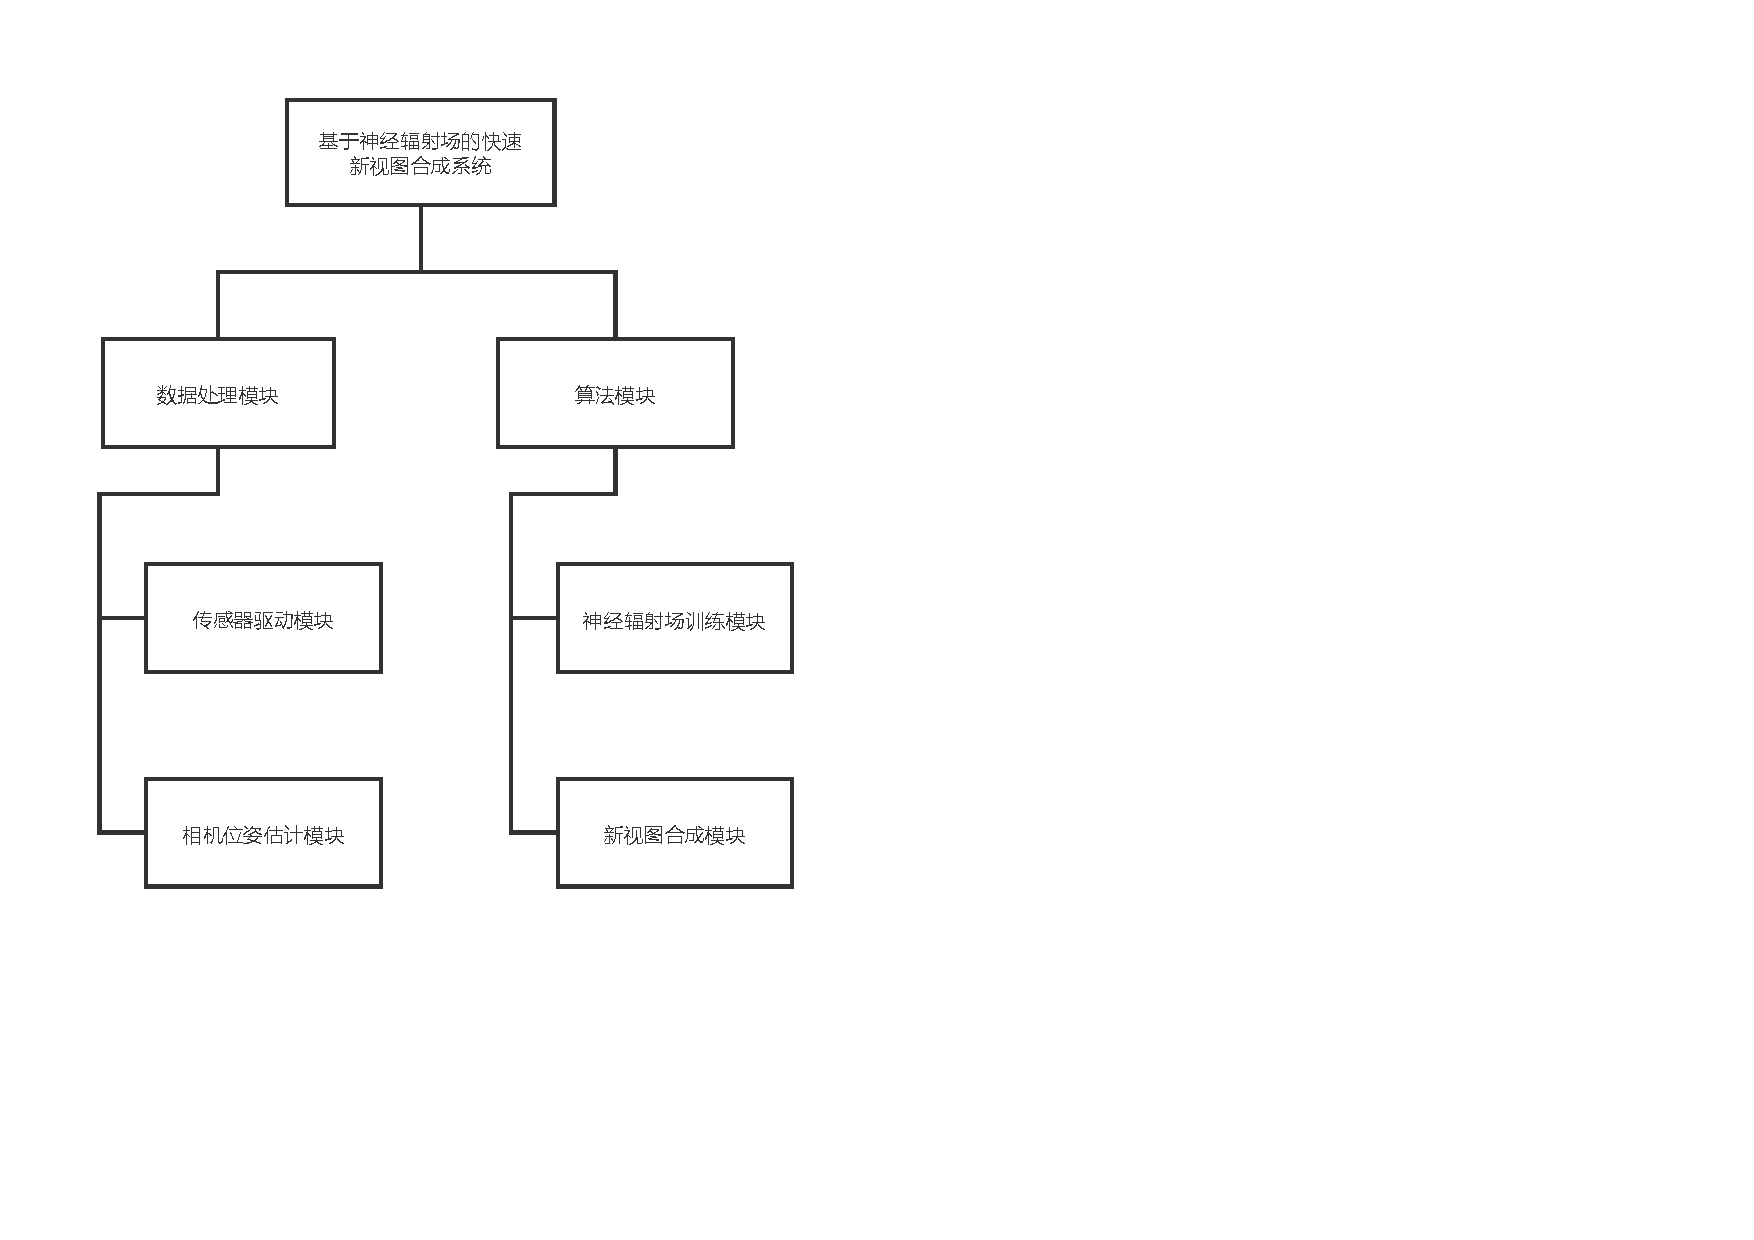
\includegraphics[width=0.65\linewidth]{figures/system_struct.pdf}
    \caption{系统功能结构图}
    \label{fig:system_struct}
\end{figure}

\begin{enumerate}
    \item [a)] 数据处理模块:包括以下两个模块内容:
               \begin{enumerate}
                   \item [1)] 传感器驱动模块:用于获取传感器的数据,例如 RGB 图像。
                   \item [2)] 相机位姿估计模块:使用 COLMAP \cite{schonberger2016structure} 实现对真实图像位姿的计算。
               \end{enumerate}
    \item [b)] 算法模块:包括以下两个模块内容:
               \begin{enumerate}
                   \item [1)] 神经辐射场训练模块:用于将已知位姿的图像训练成一个 5D 神经辐射场。
                   \item [2)] 新视图合成模块:通过训练好的模型,给定位姿,合成该位姿下的新视图。
               \end{enumerate}        
\end{enumerate}

\subsection{其他需求分析}
在经典的软件质量模型 “FURPS+” 中,除了上一小节的功能性需求,还剩下四个非功能性需求,分别是易用性 (Usability)、可靠性 (Reliability)、性能 (Performance) 还有可支持性 (Supportability)。使用 “FURPS+” 模型来实现需求分析可保障用户体验,比较好地能保证系统的运行质量。

以下是对本系统的非功能性需求进行分析:
\begin{enumerate}
    \item [a)] 易用性:在设计该系统的时候,系统的界面应该整洁美观,按钮名称应该通俗易懂,符合用户的操作习惯,降低用户的学习成本。
    \item [b)] 可靠性:系统应该足够鲁棒,能够处理各个模块中可能产生的异常,尽可能避免系统崩溃,如出现不可避免的错误应及时反馈给用户。     
    \item [c)] 性能:系统应在相关的平台上能流畅运行,系统的时延要能满足一般用户体验,本身应增加与用户交流的对话框,提高用户体验。此外,性能还体现在合成新视图的速度以及质量上,这是本文方法论所主要考量的指标。
    \item [d)] 可支持性:系统各功能模块清晰明确,模块之间应该是解耦的,方便日后维护、扩展、更新。接口命名以及教程足够清晰,方便其他开发者使用。
\end{enumerate}

\subsection{主要用例分析}
本小节主要介绍 PC 端的各个应用模块用例。

用户可以进行的操作包括与相机的交互,数据集的处理,以及新视图合成。用例图见图~\ref{fig:PCusercase}。

\pagebreak
\begin{figure}[htb]
	\centering
	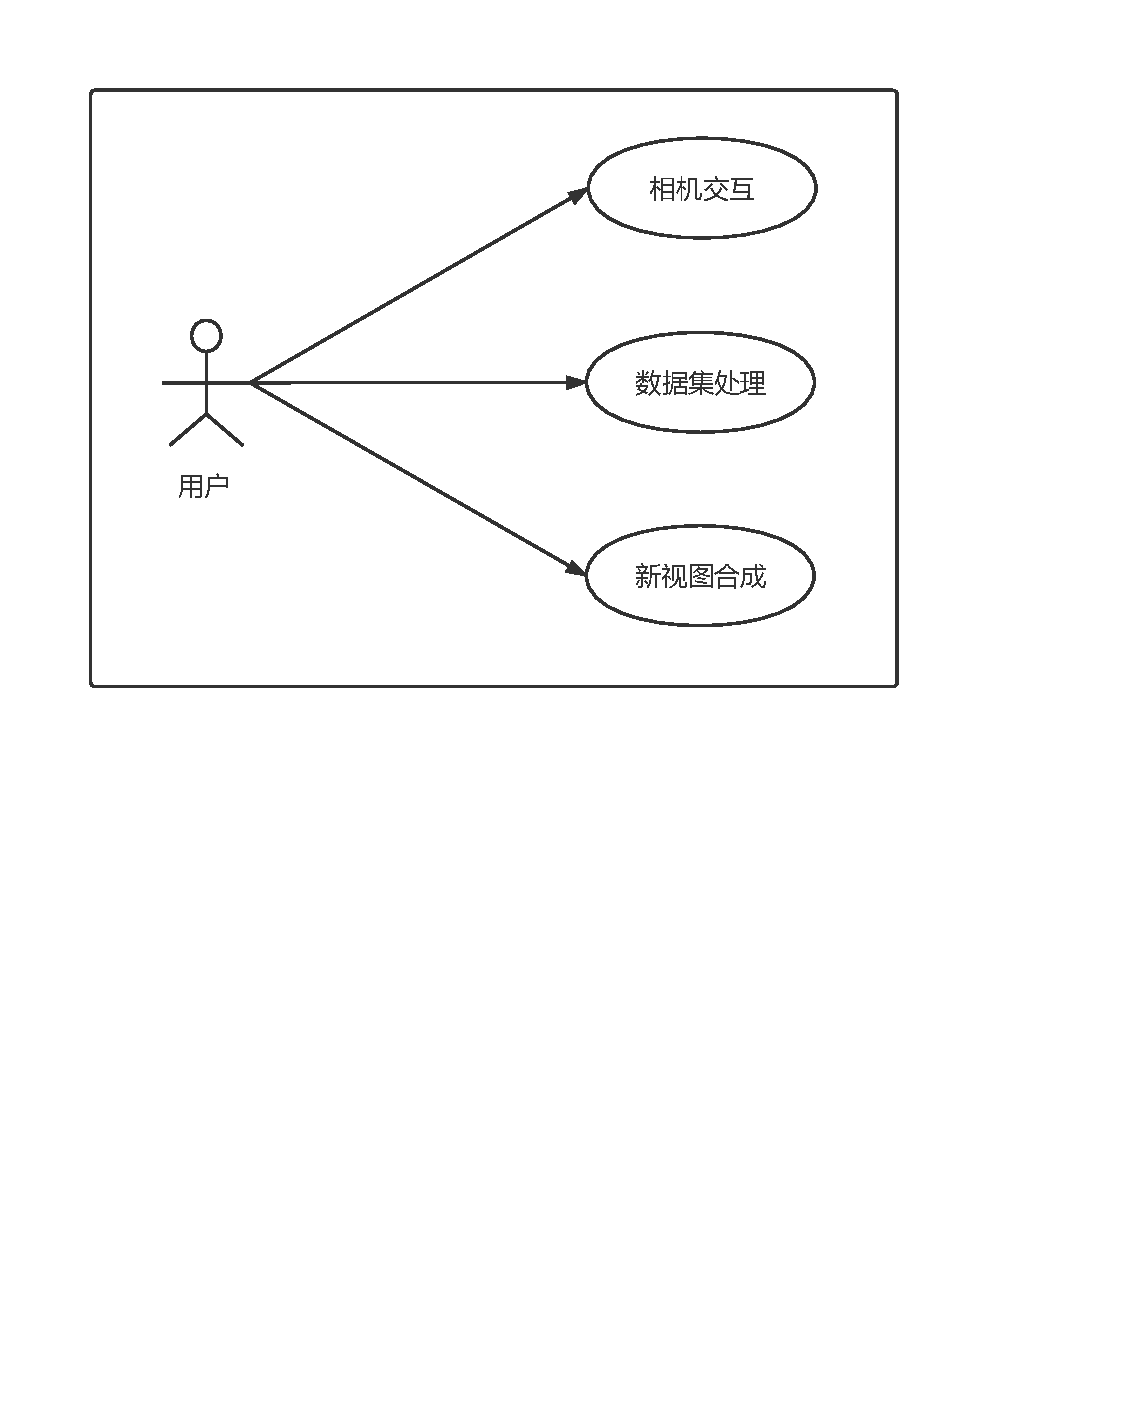
\includegraphics[width=0.55\linewidth]{figures/usercase.pdf}
	\caption{PC 客户端用例图}
	\label{fig:PCusercase}
\end{figure}

\begin{table*}
	\centering
	\small\def\arraystretch{0.91}\setlength\tabcolsep{0.05\textwidth}
	\caption{相机交互用例图User case\#1}
	\begin{tabular}{p{3.5cm}|p{8cm}}
		\hline
		用例编号 & User case\#1 \\
		\hline
		用例名 & 相机交互  \\
		\hline
		涉众及其关注点 & 用户:希望进行相机交互功能  \\
		\hline
		前置条件 & 用户启动应用 \\
		\hline
		主成功场景 & 1. 用户打开应用,点击“打开相机”按钮  \\
		& 2. 应用跳转至相机界面 \\
		& 3. 用户点击添加按钮 \\
		& 4.  当前相机画面被捕获到数据集栏并显示\\
		& 5.  用户点击“关闭相机”按钮\\
		&\quad 5a. 系统提示 “您确定要关闭相机吗?”  \\
		&\quad 5b. 系统保存用户处理结果,相机画面终止  \\
		& 6.  用户点击“退出系统”按钮\\
		&\quad 6a. 系统提示 “您确定要退出系统吗?”  \\
		&\quad 6b. 系统保存用户处理结果,整个应用退出  \\
		\hline
		拓展 & 5a. 相机关闭取消  \\	
		 & \quad 1. 交互界面保持不变  \\	
		     & 6a. 系统关闭取消  \\	
		& \quad 1. 交互界面保持不变  \\		
		\hline
		后置条件 & 应用显示相应处理结果 \\
		\hline
		发生频率 & 高 \\
		\hline
	\end{tabular}
	\label{tab:usercase1}
\end{table*}

\begin{table*}[thbp]
	\centering
	\small\def\arraystretch{1.5}\setlength\tabcolsep{0.05\textwidth}
	\caption{数据集处理用例图User case\#2}
	\begin{tabular}{p{3.5cm}|p{8cm}}
		\hline
		用例编号 & User case\#2 \\
		\hline
		用例名 & 数据集处理  \\
		\hline
		涉众及其关注点 & 用户:希望数据集处理功能  \\
		\hline
		前置条件 & 用户启动应用 \\
		\hline
		主成功场景 & 1. 用户打开应用,点击“打开相机”按钮  \\
		& 2. 应用跳转至相机界面 \\
		& 3. 用户点击添加按钮 \\
		& 4.  当前相机画面被捕获到数据集栏并显示\\
		& 5.  用户在数据集栏点击“上(下)一张”按钮\\
		& 6.  用户在数据集栏点击“删除”按钮\\
		&\quad 6a. 系统提示 “您确定删除吗?”  \\
		&\quad 6b. 系统保存用户处理结果,当前图像被删除  \\
		\hline
		拓展 & 3a. 添加数据集前未打开相机  \\	
		& \quad 1. 弹出提示框“请打开相机”  \\
		& 5a. 数据集为空  \\	
		& \quad 1. 弹出提示框“请添加图像至数据集”  \\
		& 6a. 点击取消删除或提示栏右上角$\times$  \\	
		& \quad 1. 数据集栏当前画面被保留  \\
		& 6b. 删除时,数据集为空$\times$  \\	
		& \quad 1. 弹出提示框“不可删除空数据”  \\	
		\hline
		后置条件 & 应用显示相应处理结果 \\
		\hline
		发生频率 & 高 \\
		\hline
	\end{tabular}
	\label{tab:usercase2}
\end{table*}

\begin{table*}[thbp]
	\centering
	\small\def\arraystretch{1.7}\setlength\tabcolsep{0.05\textwidth}
	\caption{新视图合成用例图User case\#3}
	\begin{tabular}{p{3.5cm}|p{8cm}}
		\hline
		用例编号 & User case\#3 \\
		\hline
		用例名 & 新视图合成  \\
		\hline
		涉众及其关注点 & 用户:希望执行新视图合成功能  \\
		\hline
		前置条件 & 用户启动应用 \\
		\hline
		主成功场景 & 1. 用户点击“计算位姿”按钮  \\
		& 2. 进度条提示计算位姿的过程 \\
		& 3. 用户点击“训练模型”按钮 \\
		& 4.  进度条提示模型训练的过程\\
		& 5.  用户点击“合成新视图”按钮\\
	    & 6. 状态提示从“待合成”到“合成中”再到“已合成” \\
	    & 7. 用户在数据集栏点击“上(下)一张”按钮 \\
		\hline
		拓展 & 1a. 计算位姿时,数据集为空:  \\	
		& \quad 1.   弹出提示框:“数据集不能为空”\\
		& 3a. 训练模型时,位姿为空:  \\	
		& \quad 1.   弹出提示框:“请先计算位姿”\\
		& 5a. 训练模型时,未训练模型:  \\	
		& \quad 1.   弹出提示框:“请先训练模型”\\		
		\hline
		后置条件 & 应用显示相应处理结果 \\
		\hline
		发生频率 & 高 \\
		\hline
	\end{tabular}
	\label{tab:usercase3}
\end{table*}

\pagebreak	
\section{系统设计}

\subsection{系统架构设计}
本文提出的神经辐射场的新视图快速合成系统主要分为三个部分,包含界面层、业务层、数据层。其中,界面层主要是为用户提供可视化的应用界面以方便用户进行相应的操作。业务层提供了本系统的所有业务基本操作,包括传感器驱动、位姿估计、神经辐射场训练、新视图合成。数据层负责数据库的管理和数据的控制,通过相机获取一系列 RGB 图像,并传给业务层去处理下游任务。本文系统是基于 Windows 平台的应用,对应的 PC 客户端使用 matlab 的 App Design 工具箱实现,具体的系统架构如图~\ref{fig:symtem_design} 所示。

\begin{figure}[htbp]
	\centering
	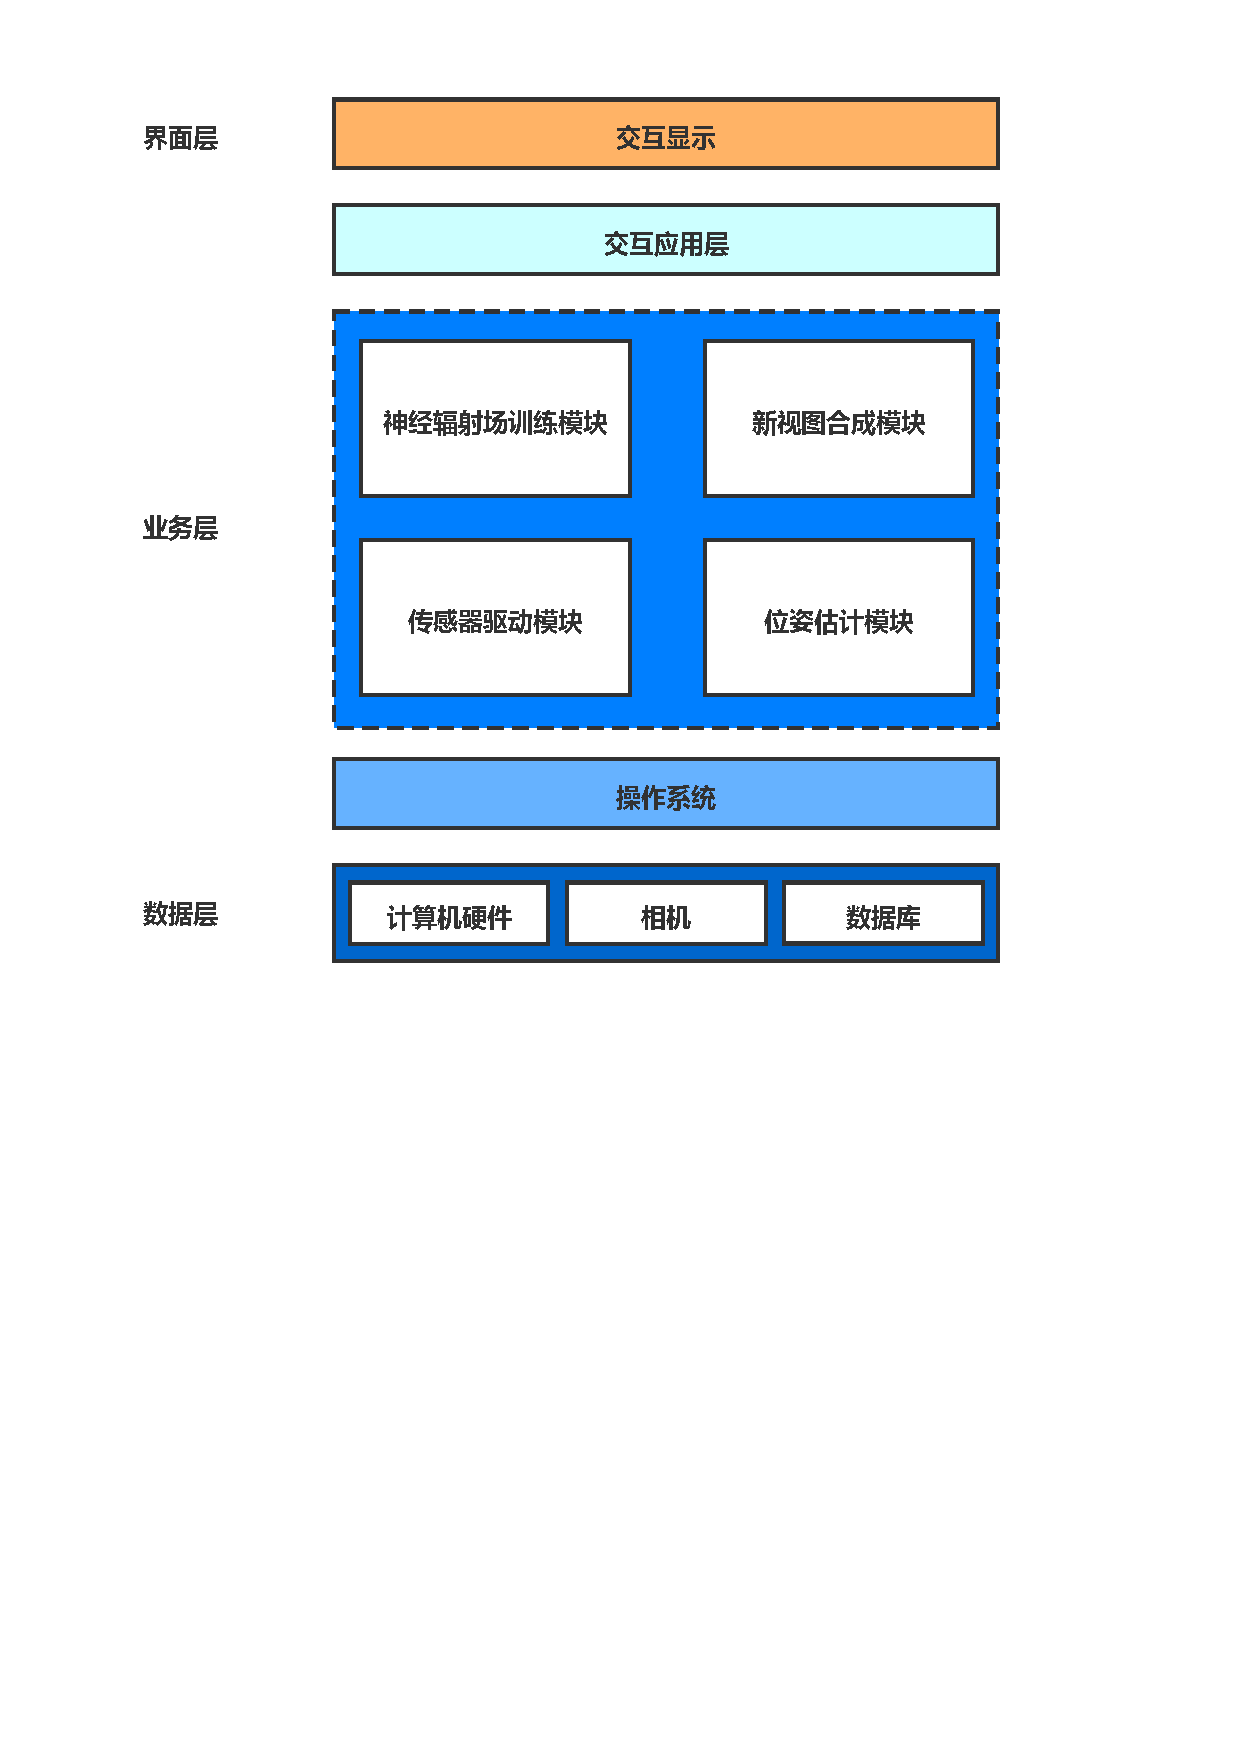
\includegraphics[width=0.75\linewidth]{figures/system_design_revised.pdf}
	\caption{系统架构示意图}
	\label{fig:symtem_design}
\end{figure}

\subsection{关键用例实现}
\subsubsection{相机交互}
相机交互功能的具体交互流程如下:
\begin{enumerate}
	\item 用户点击“打开相机”按钮,系统通过 MainWindow 激活 SensorDrive ,打开相机。
	
	\item 用户点击“添加”按钮,系统通过 SensorDrive 捕获实时的相机画面,一方面将调用 SensorDrive 的方法 addViewClicked,另一方面将该画面返回 MainWindow 并显示。
	\item 用户点击“关闭相机”按钮,系统通过 SensorDrive 关闭相机,并显示在 MainWindow 上。 
\end{enumerate}

图~\ref{fig:cameraSD} 是相机交互的顺序图,描述了上述交互流程。

\begin{figure}[htbp]
	\centering
	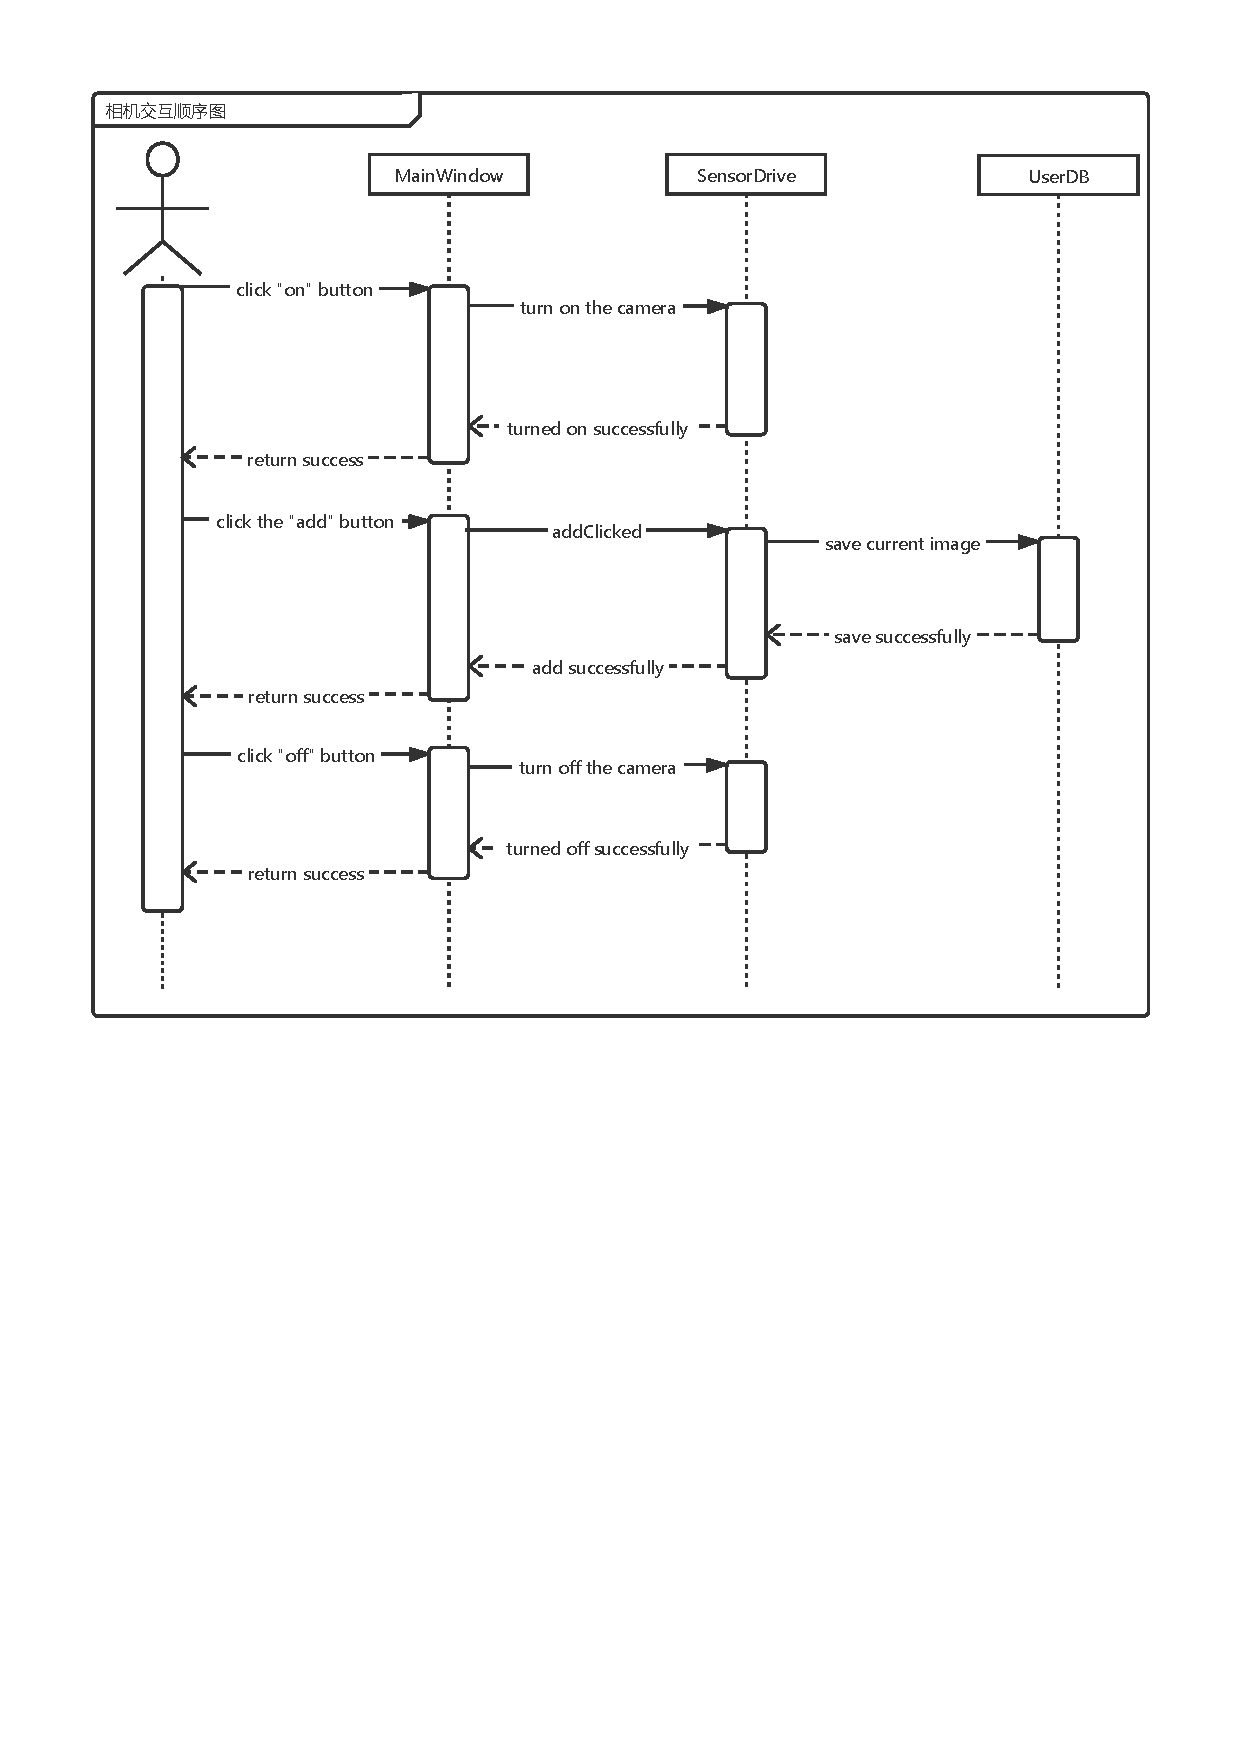
\includegraphics[width=0.85\linewidth]{figures/cameraSD.pdf}
	\caption{相机交互顺序图}
	\label{fig:cameraSD}
\end{figure}

\subsubsection{数据集处理}

\begin{enumerate}
	\item 用户点击“打开相机”按钮,系统通过 MainWindow 激活 SensorDrive ,打开相机。
	
	\item 用户点击“添加”按钮,系统通过 SensorDrive 捕获实时的相机画面,一方面将调用 SensorDrive 的方法 addViewClicked,另一方面将该画面返回 MainWindow 并显示。
	
	\item 用户点击“上/下一张”按钮,系统调用 UserDB 中的接口 lastClicked/nextClicked,系统将结果返回 MainWindow。
	
	\item 用户点击“删除”按钮,系统调用 UserDB 中的接口 deleteClicked,系统将结果返回 MainWindow。
\end{enumerate}

\begin{figure}[htbp]
	\centering
	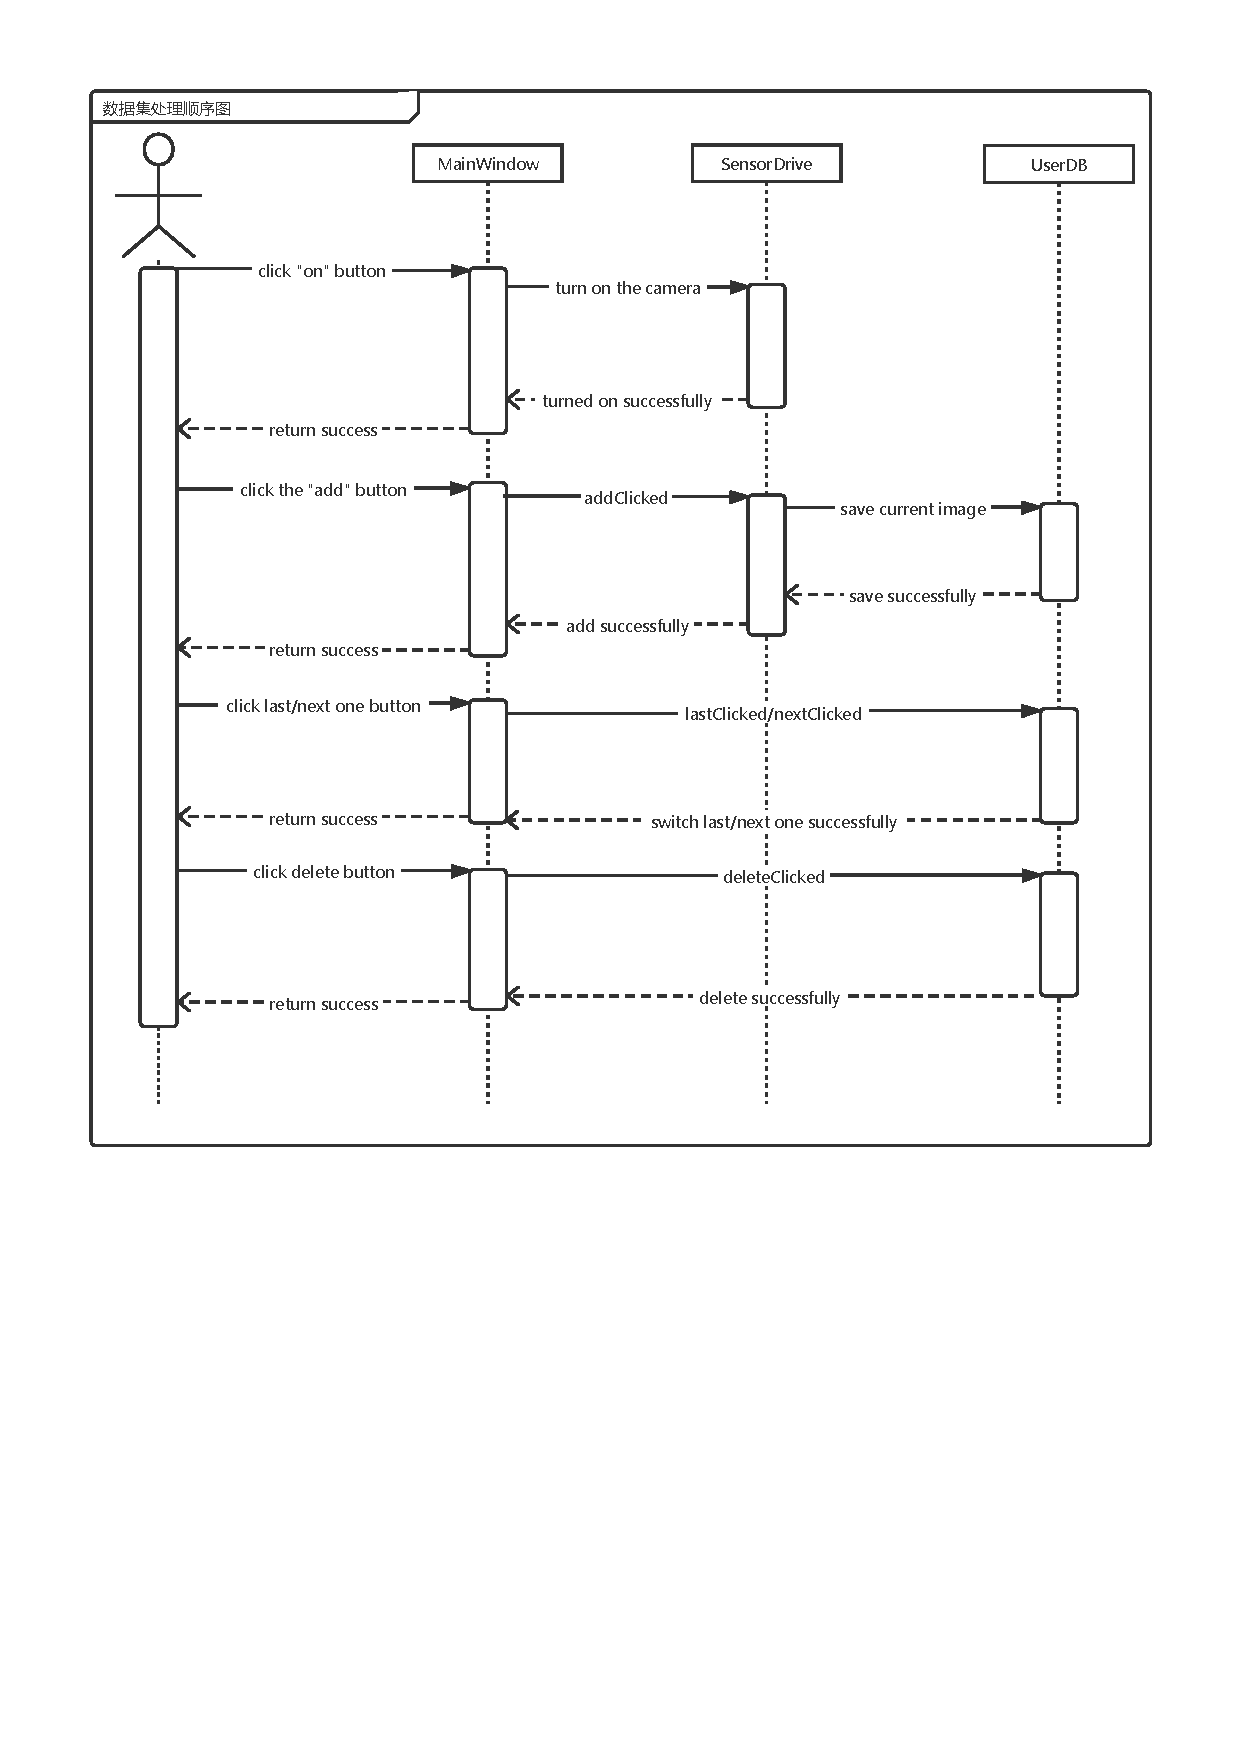
\includegraphics[width=0.85\linewidth]{figures/datasetProcessSD.pdf}
	\caption{数据集处理顺序图}
	\label{fig:datasetProcessSD}
\end{figure}

图~\ref{fig:datasetProcessSD} 是数据集处理的顺序图,描述了上述交互流程。

\subsubsection{新视图合成}
\begin{enumerate}
	\item 用户点击“计算位姿”按钮,系统通过 calPosesClicked 激活 FNeRF,打开相机。
	
	\item 用户点击“训练模型”按钮,系统通过 trainNeRFClicked 激活 FNeRF 使之向 UserDB 请求相应的数据并开始训练,训练过程进度条将显示在 MainWindow 上。
	
	\item 用户点击“合成新视图”按钮,系统通过 synViewsClicked 激活 FNeRF 使之向 UserDB 请求相应网络参数并开始渲染新视图,合成完毕信息将显示在 MainWindow 上。
\end{enumerate}

\begin{figure}[htbp]
	\centering
	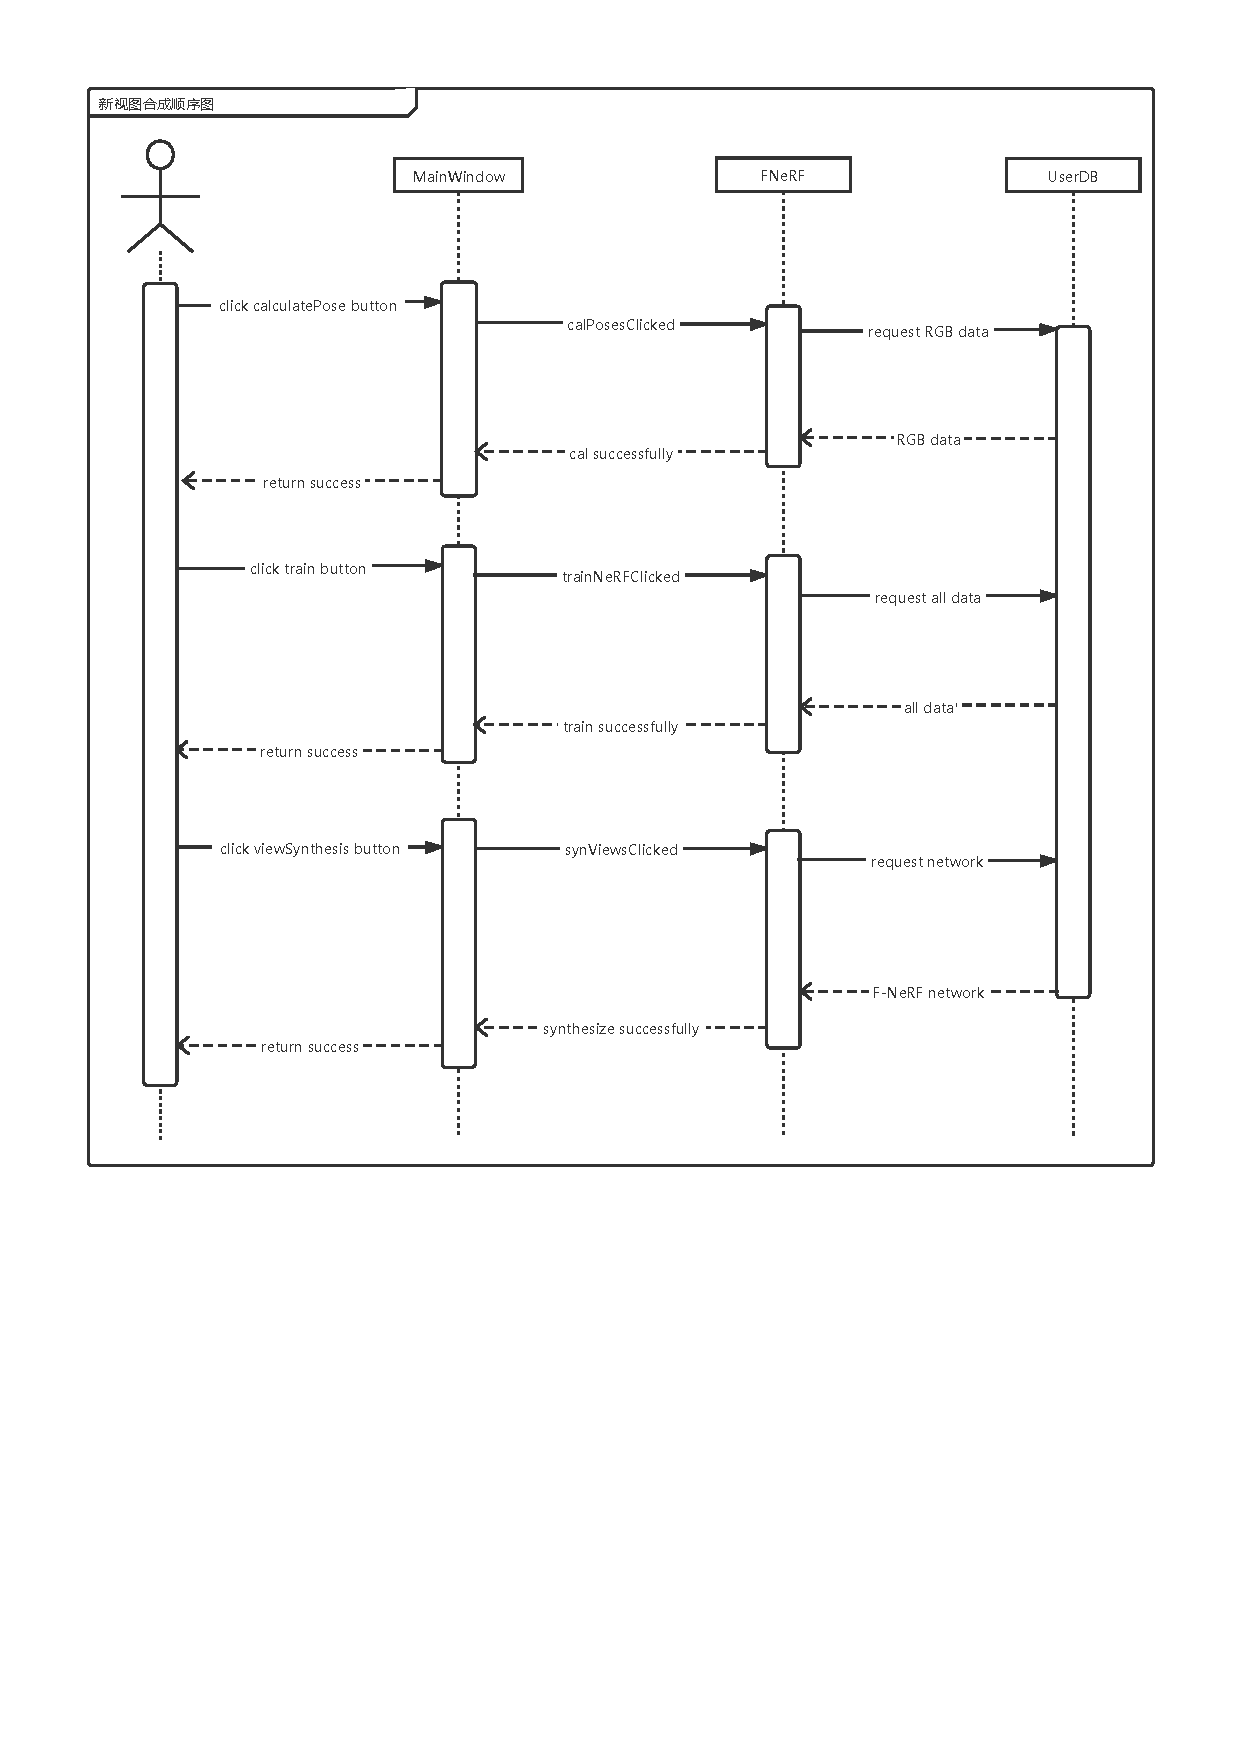
\includegraphics[width=0.85\linewidth]{figures/viewSynthesisSD.pdf}
	\caption{新视图合成顺序图}
	\label{fig:viewSynthesisSD}
\end{figure}

图~\ref{fig:viewSynthesisSD} 是新视图合成的顺序图,描述了上述交互流程。

\pagebreak
\subsection{模块详细设计}
\subsubsection{整体模块结构}
本系统主要由传感器驱动模块、位姿估计模块、神经辐射场训练模块以及新视图合成模块组成。这些模块的基本功能在第~\ref{functional} 小节已经简要叙述。
\subsubsection{传感器驱动模块}
传感器驱动模块实际上在本文中指的是相机模块,用以获取传感器的数据例如 RGB 图像,具体的类图如图~\ref{fig:sensorDriveCD} 所示。其中,MainActivity 为用户操作的主页面类,SensorActivity 为传感器操作类,ViewObject 封装了包含图像、位姿等信息的类。在 MainActivity 中打开相机后,系统调用 SensorActivity 的方法 addViewClicked 以捕获当前相机的画面,并通过 sendImage 在主界面显示当前捕获的图像,并将该图像存储在 UserDB 中。
\begin{figure}[htbp]
	\centering
	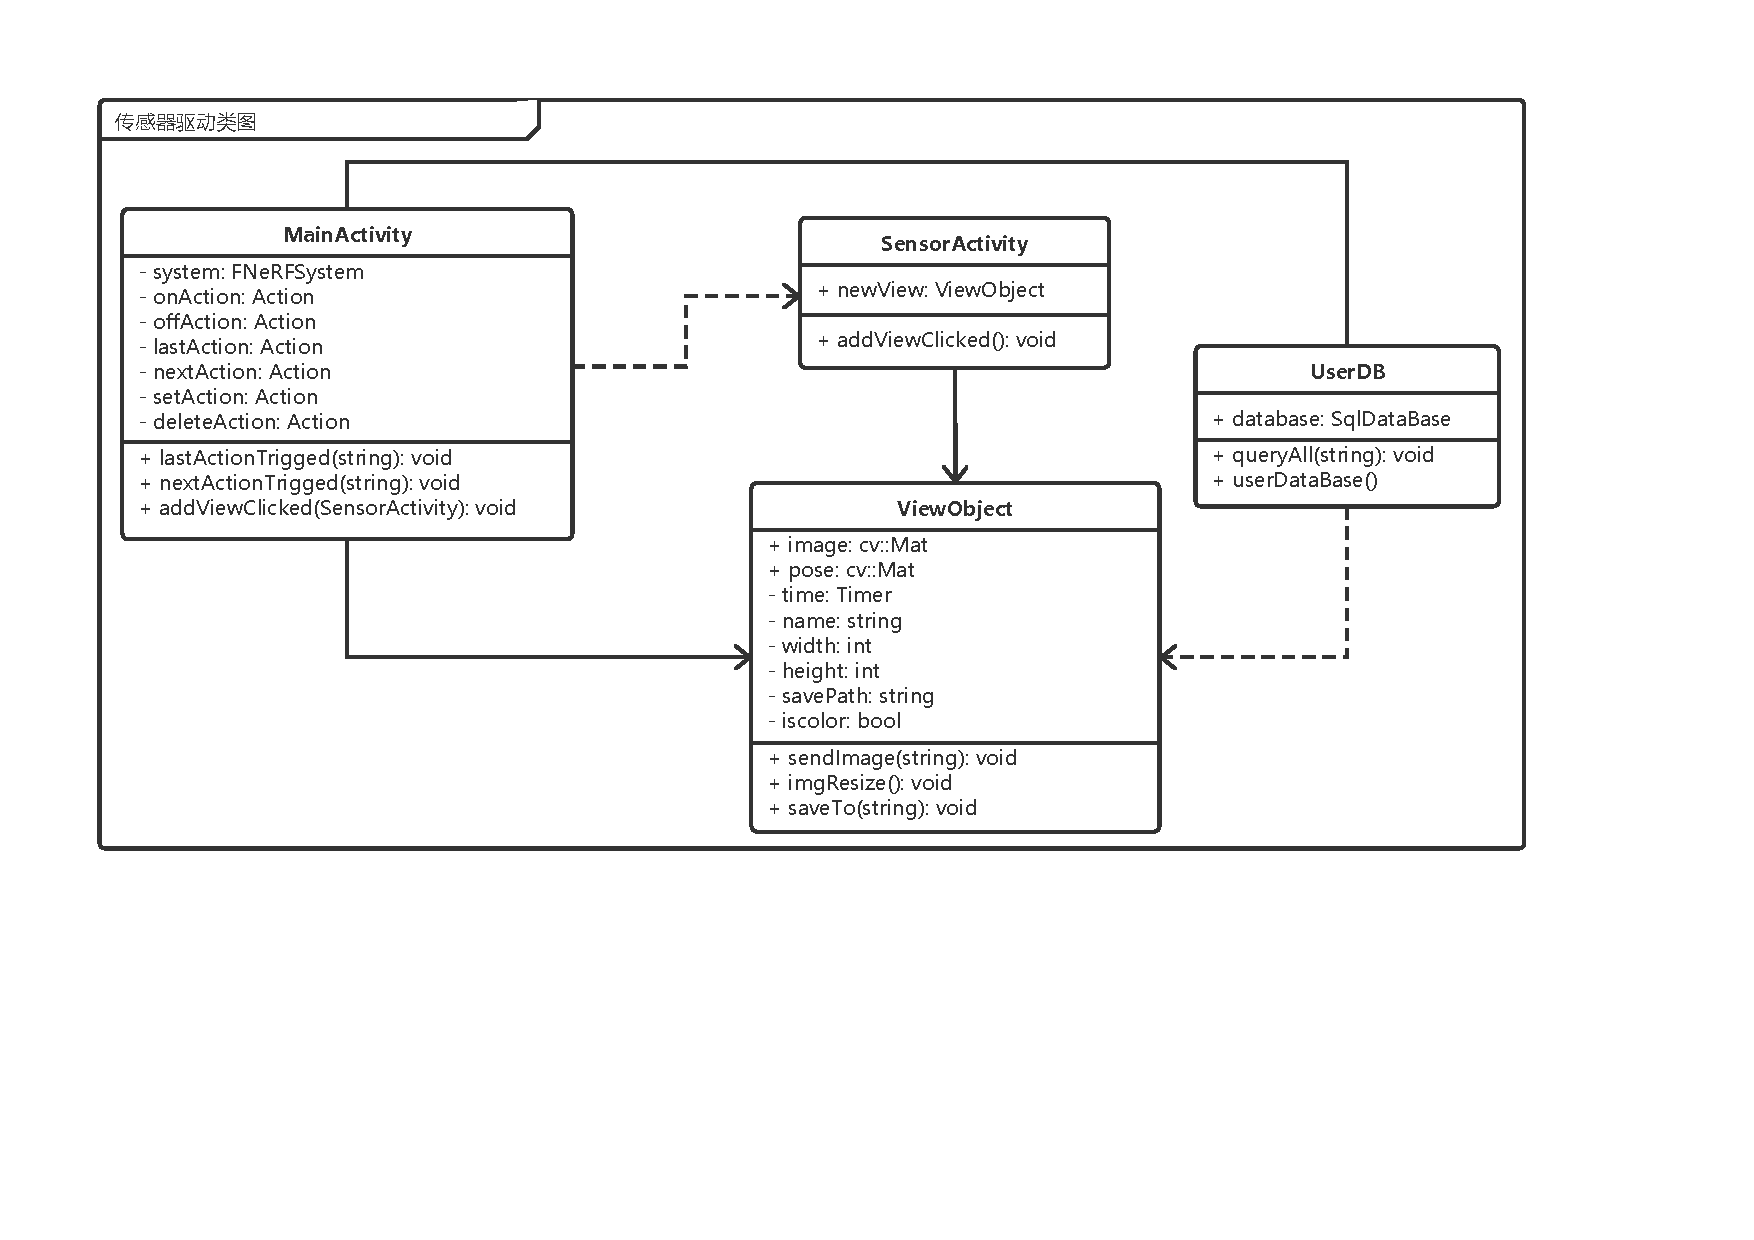
\includegraphics[width=0.95\linewidth]{figures/sensorDriveCD.pdf}
	\caption{传感器驱动类图}
	\label{fig:sensorDriveCD}
\end{figure}
\pagebreak
\subsubsection{位姿估计模块}
位姿估计模块在本系统中起着预处理数据的作用,调用 COLMAP\cite{schonberger2016structure} 算法的接口根据原始采集的 RGB 数据估计出相机位姿。

按照位姿估计模块的需求,构建了如图~\ref{fig:poseEstimationCD} 所示的类图以及方法。其中,PoseEstimator 为位姿估计模块对应的类,FNeRFSystem 为本系统各模块合并的类。通过 PoseEstimator 加载原始采集的 RGB 数据,并调用 COLMAP 的接口对位姿进行估计,之后将计算结果保存至数据库 UserDB。
\begin{figure}[htbp]
	\centering
	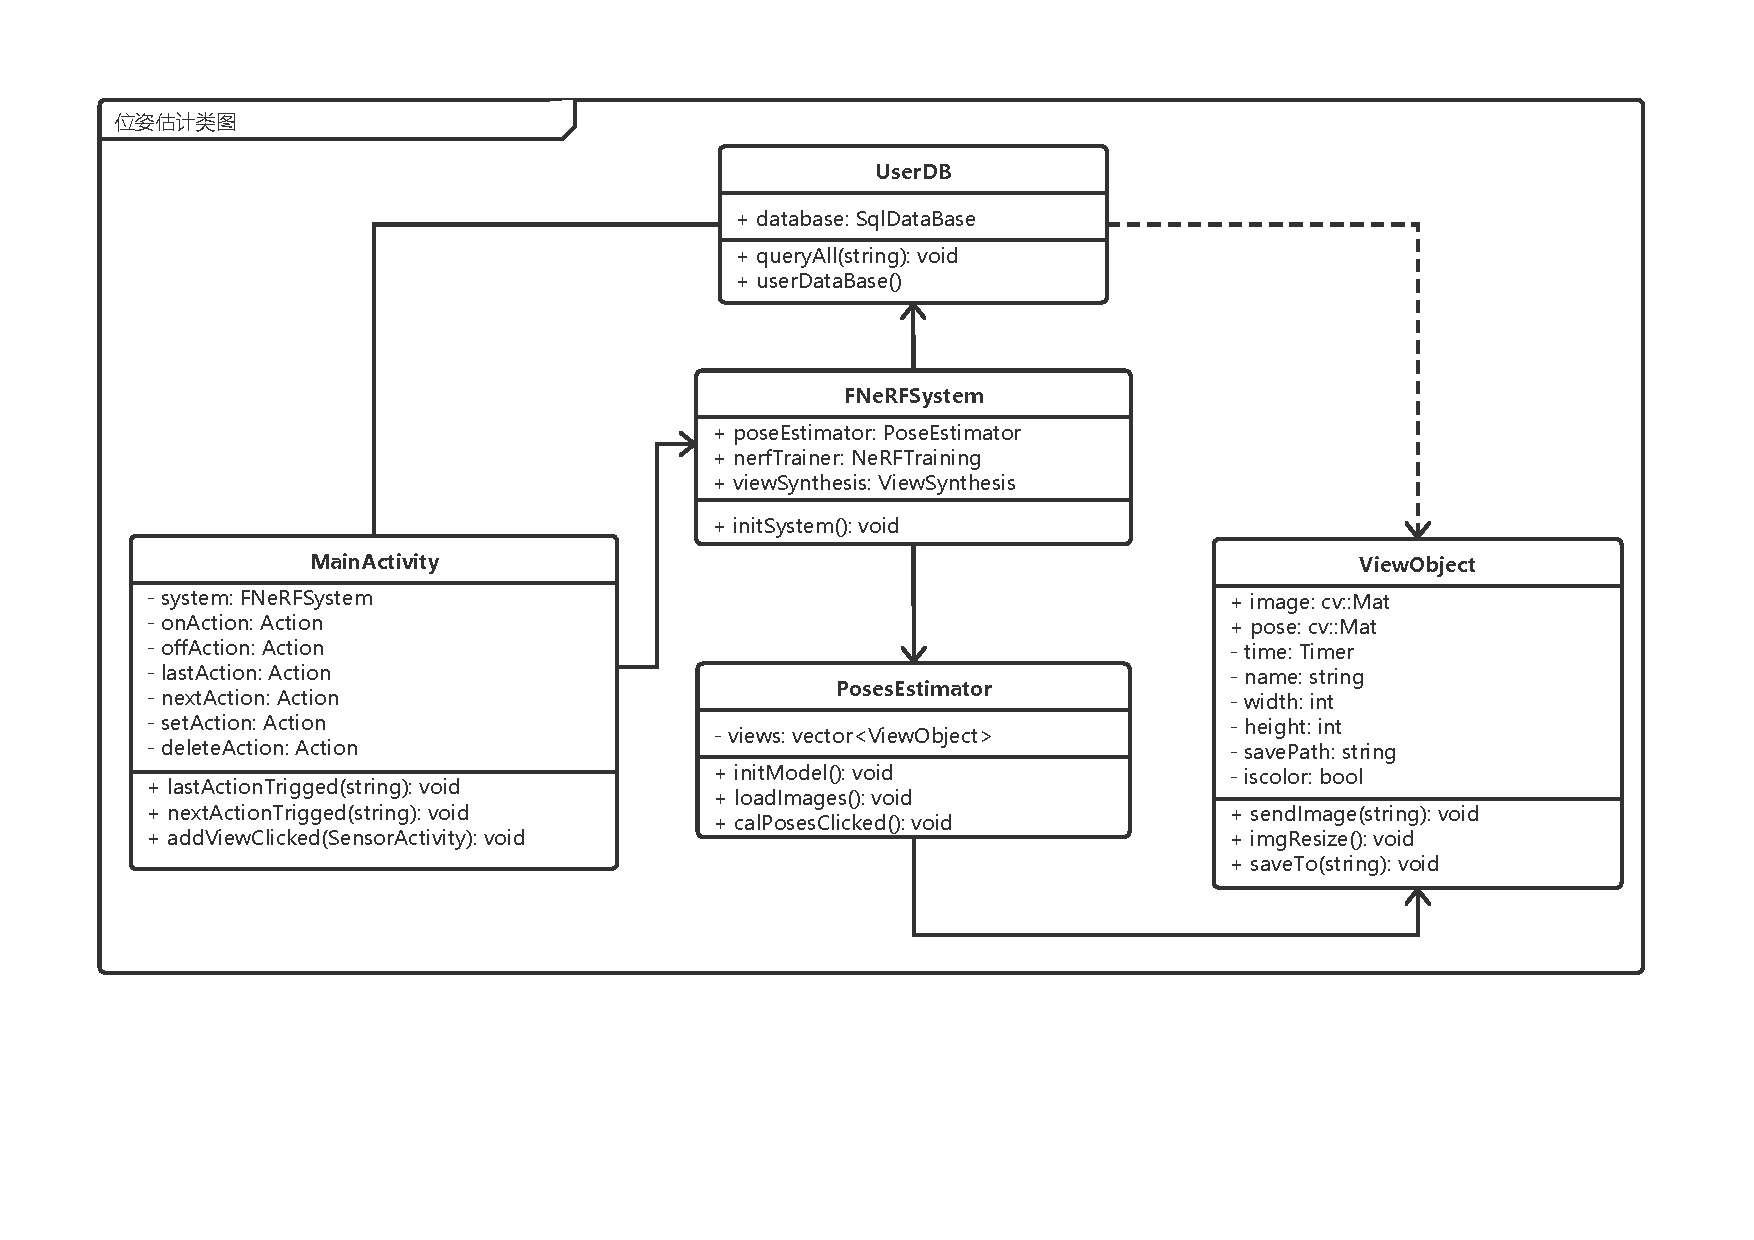
\includegraphics[width=0.95\linewidth]{figures/poseEstimationCD.pdf}
	\caption{位姿估计类图}
	\label{fig:poseEstimationCD}
\end{figure}

\subsubsection{神经辐射场训练模块}
神经辐射场训练模块实际上是使用本文第三章提出的基于神经辐射场的快速新视图合成算法对估计了位姿后的数据集进行训练,训练完毕后会保存神经网络的相关参数,便于后续快速新视图合成的测试。

根据神经辐射场训练模块的需求,构建了如图~\ref{fig:NeRFTrainCD} 所示的类图,NeRFTraining 为训练过程对应的类。通过 NeRFTraining 可以加载数据集并进行神经辐射场的训练,在训练过程中和训练完毕后都会保存相应的网络参数,便于测试时使用。
\begin{figure}[htbp]
	\centering
	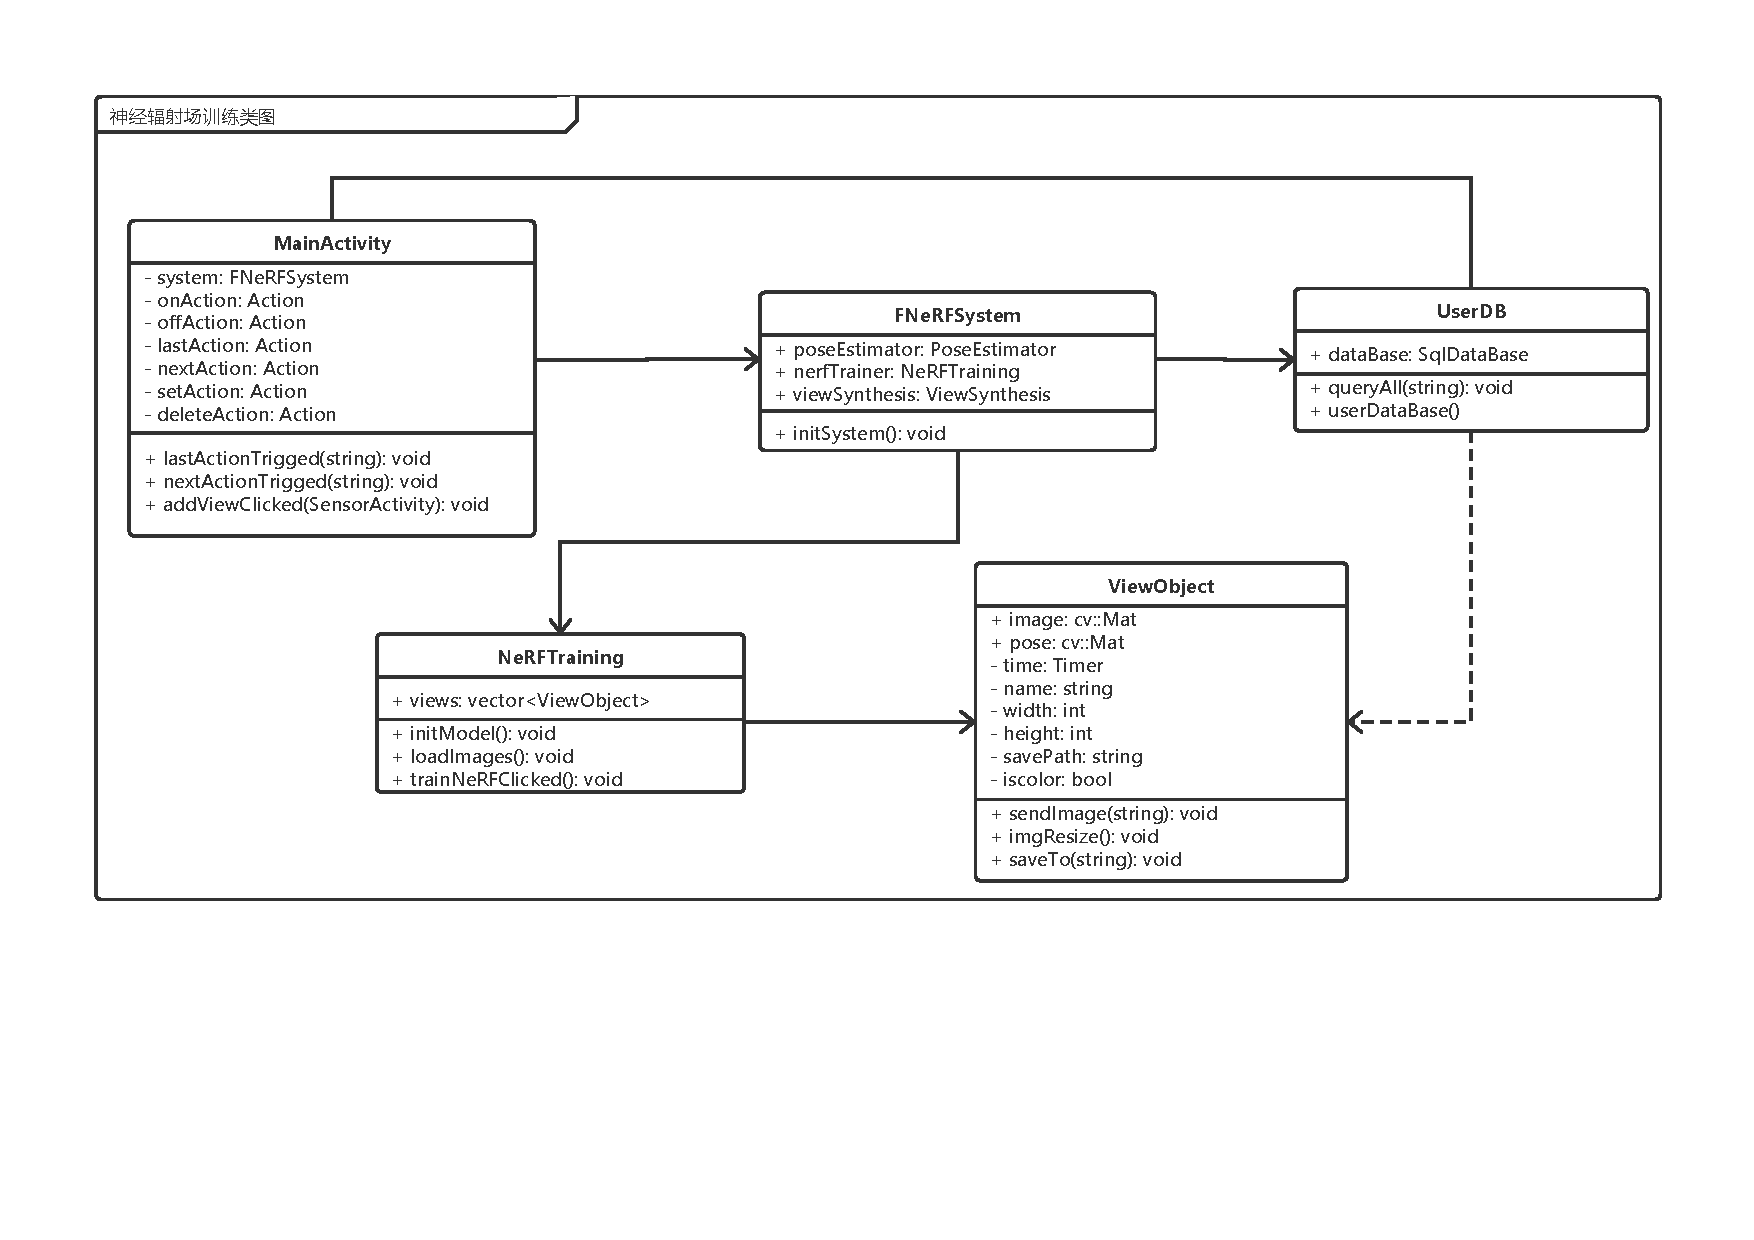
\includegraphics[width=0.95\linewidth]{figures/NeRFTrainCD.pdf}
	\caption{神经辐射场训练类图}
	\label{fig:NeRFTrainCD}
\end{figure}
\subsubsection{新视图合成模块}
新视图合成模块也是本系统的最后一个模块,负责使用训练好的神经辐射场(即 F-NeRF)快速合成新视角下的图像。

如图~\ref{fig:viewSynthesisCD} 所示的是新视图合成的类图,ViewSynthesis 对应着合成新视图的类。实际中,在测试之前需要提前加载好新视角下的位姿,然后使用 ViewSynthesis 中的 synViewClicked 方法通过训练好的 F-NeRF 网络合成新视图,并将新视图的质量和速度评价指标打印到主窗口上。
\begin{figure}[htbp]
	\centering
	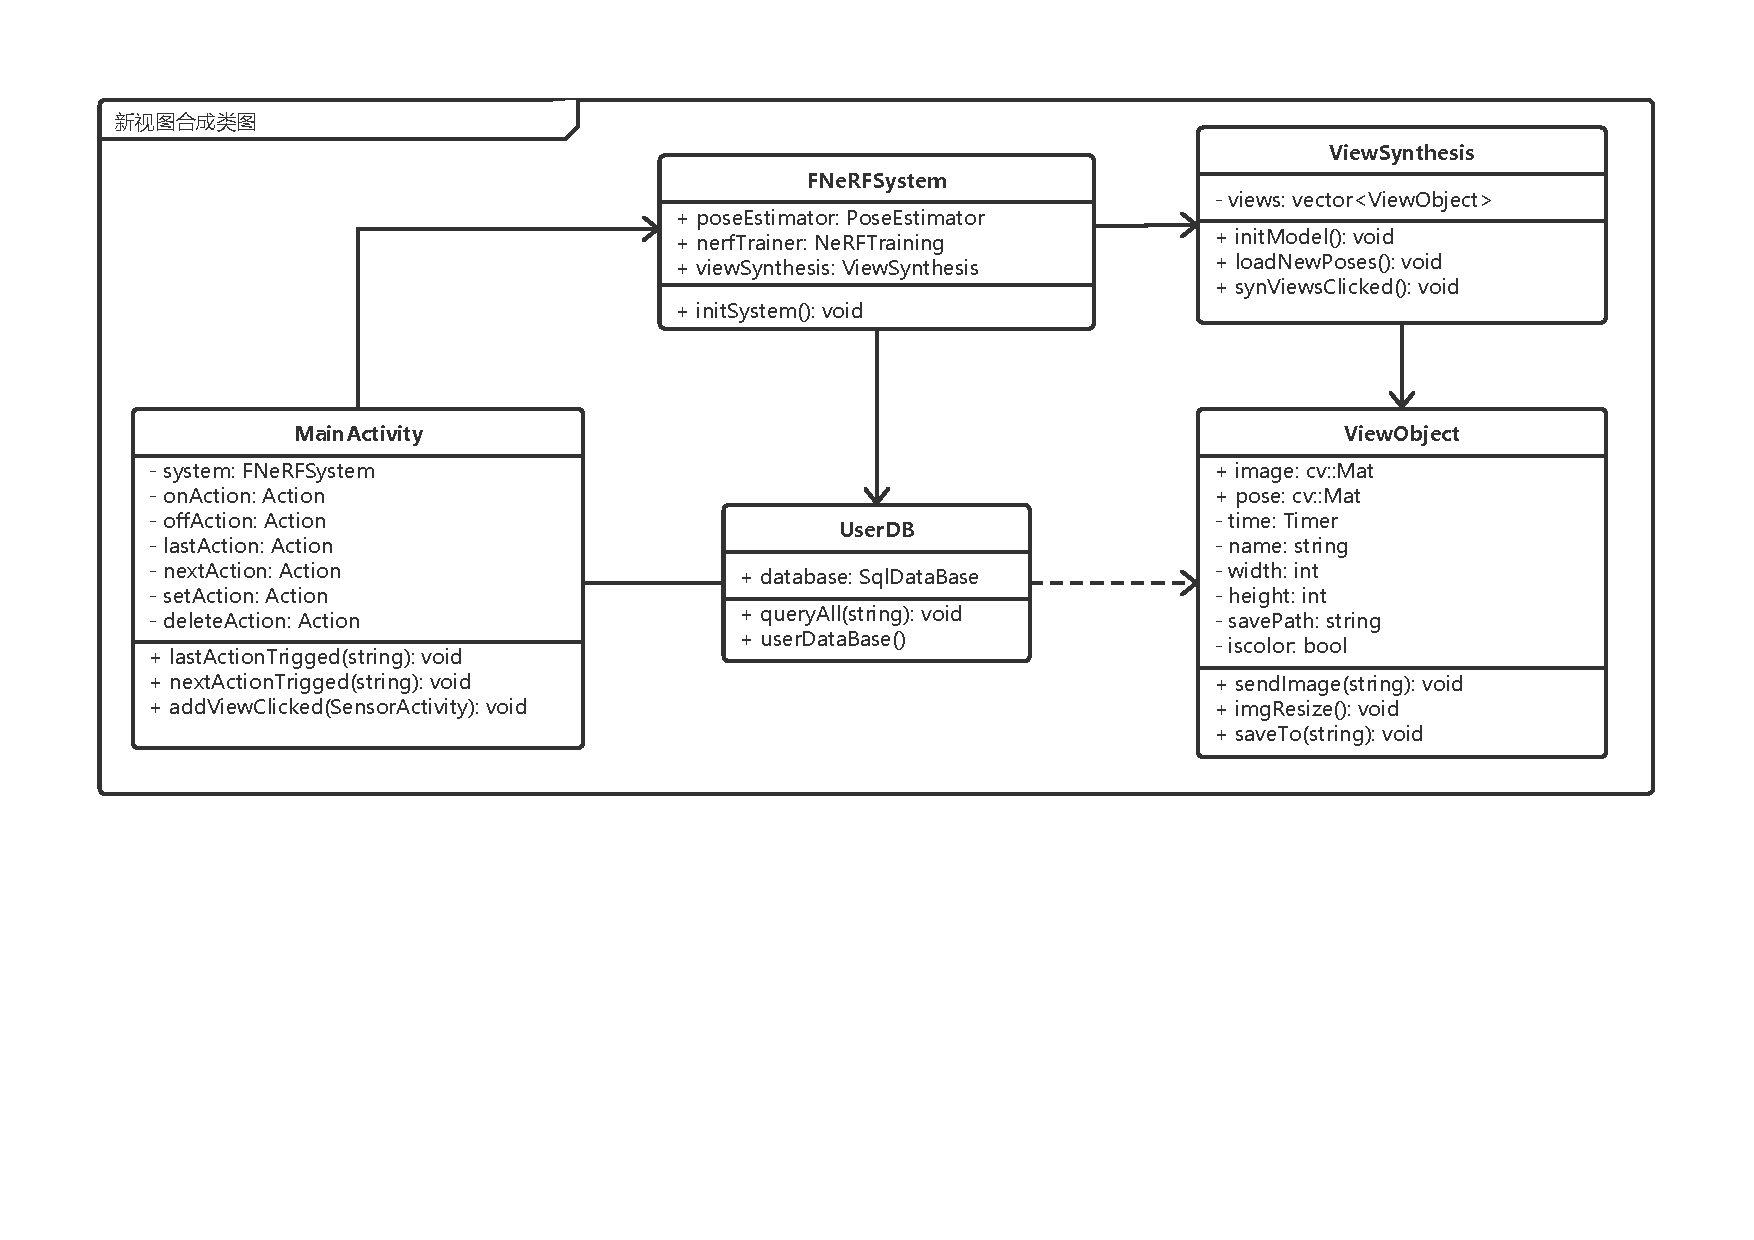
\includegraphics[width=0.95\linewidth]{figures/viewSynthesisCD.pdf}
	\caption{新视图合成类图}
	\label{fig:viewSynthesisCD}
\end{figure}

\subsection{主要技术细节实现}
本文设计并实现的基于神经辐射场的快速新视图合成系统是基于 Windows 平台开发,算法模块和数据处理模块均是基于 C++ 语言编写,用户交互界面是基于 matlab 语言编写。C++ 和 matlab 语言之间靠动态链接库进行数据通信。由于本文使用的基于神经辐射场的新视图快速合成模型是基于 Pytorch 框架训练的,而移动传感器调用代码使用的则是 C++ 语言,为了联合开发,需要引入 Pytorch 中的 torch.jit API 用来转换成 C++ 语言支持的模型文件上。

数据处理模块的位姿估计模块是基于开源的 COLMAP 框架去估计真实世界图像的位姿的,当然这不会像合成数据集那样有绝对准确的位姿,质量这一部分势必会下降,但位姿的优化不是本文所研究的问题,在此不作过多阐述。接下来将详细介绍本文快速新视图合成算法模块的 Pytorch 模型是如何移植到 C++ 代码上的,需要使用到 LibTorch 库。

Pytorch 是 Facebook 于2007年开发的当今最流行的深度学习框架之一。它有许多优点,比如底层使用 C++ 语言编写,有类似于 numpy 的张量计算,可以用于 GPU 加速,并且支持动态图,编写调试灵活,深受深度学习开发人员的青睐。为了将 pytorch 训练好的模型能够方便地迁移到 C++ 代码中,需要使用 Pytorch 的 C++ API 模型文件 LibTorch。模型转换加载的过程如下: 

\begin{enumerate}
    \item 首先是模型转换,创建与模型相同的随机张量,使用 torch.jit.trace 模块对运算过程和权值进行跟踪和捕获,进而序列化为 LibTorch 可以加载的模型文件。
    \item 下载对应平台预编译好的 LibTorch 库,添加 include 和 lib 目录
到编译环境中。
    \item 在 C++ 代码中加载转换后的 Pytorch 模型即可调用。 
\end{enumerate}

%\begin{figure}[htb]
%    \centering
%    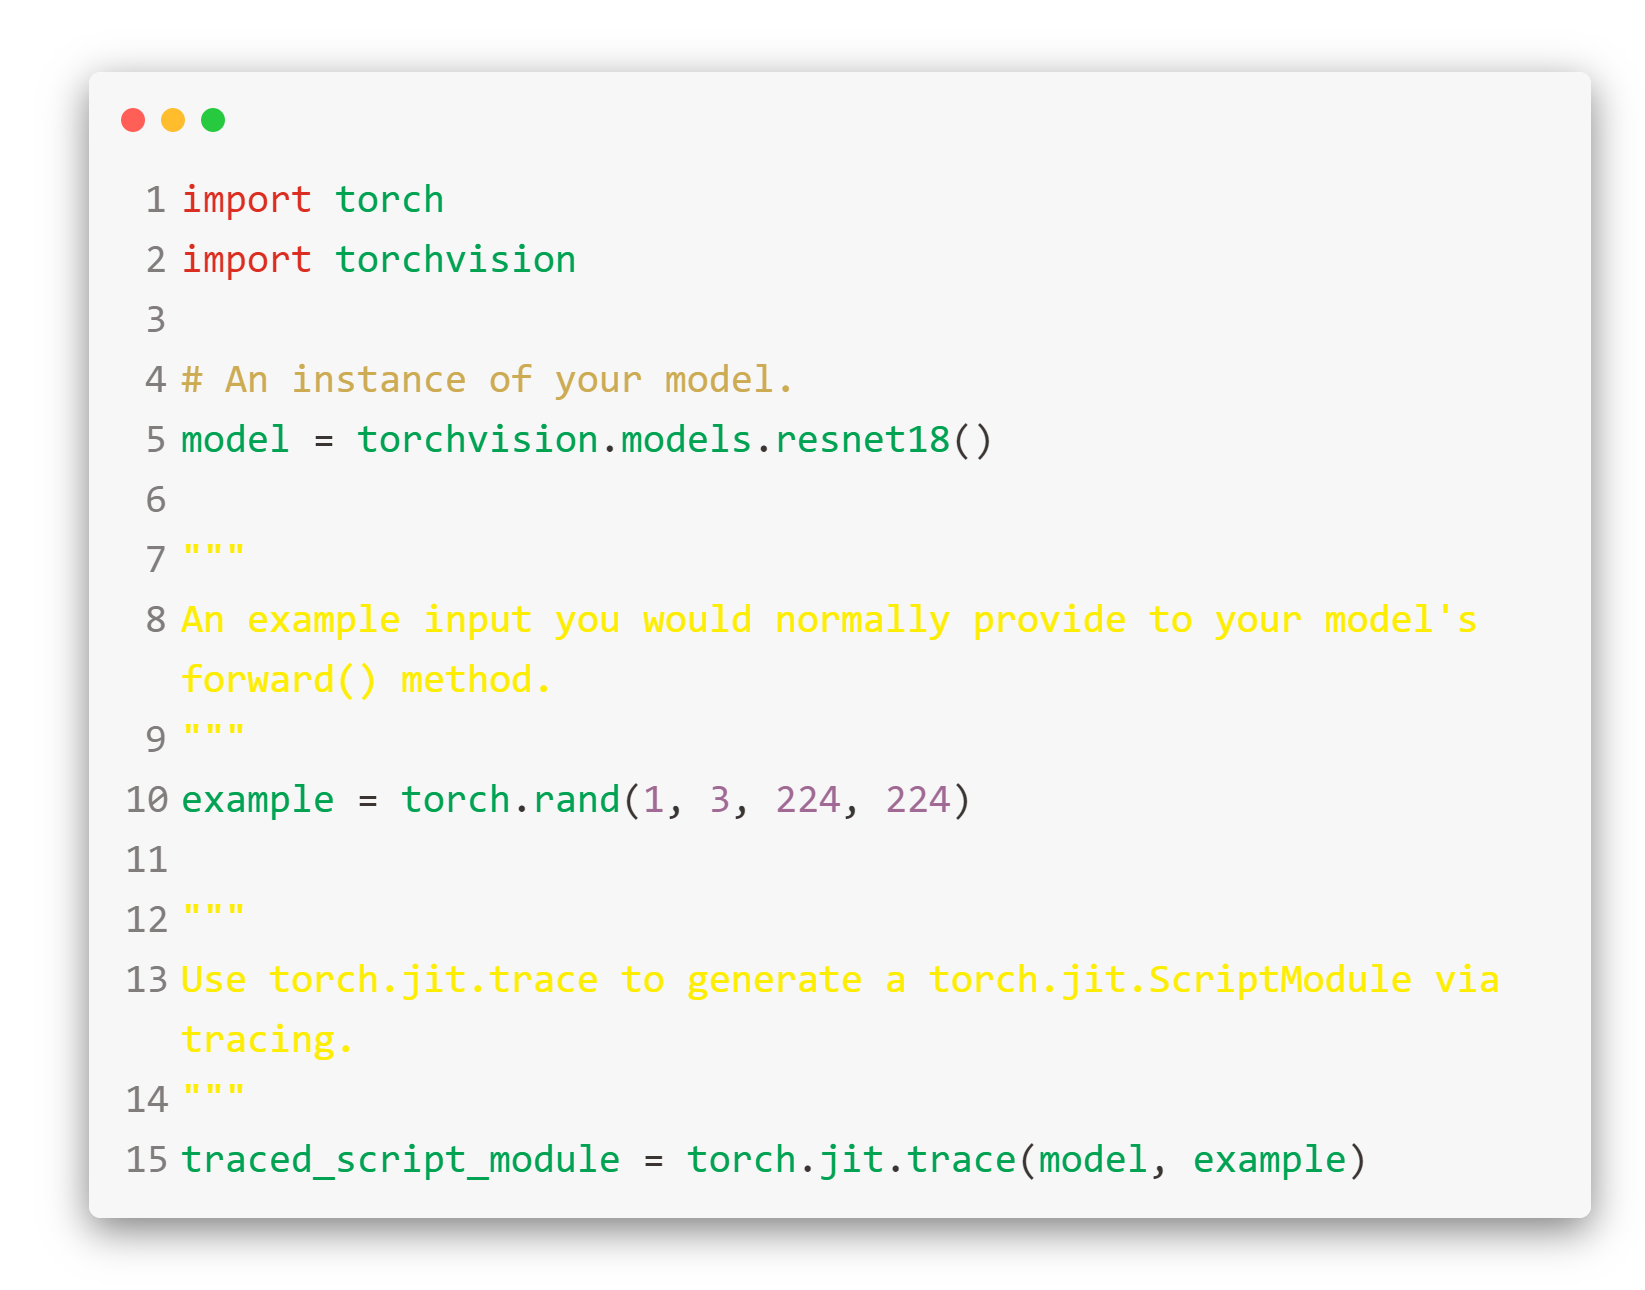
\includegraphics[width=0.98\linewidth]{figures/code-pytorch-big.png}
%    \caption{Pytorch 模型的转换}
%    \label{fig:code_pytorch}
%\end{figure}
%
%\begin{figure}[H]
%    \centering
%    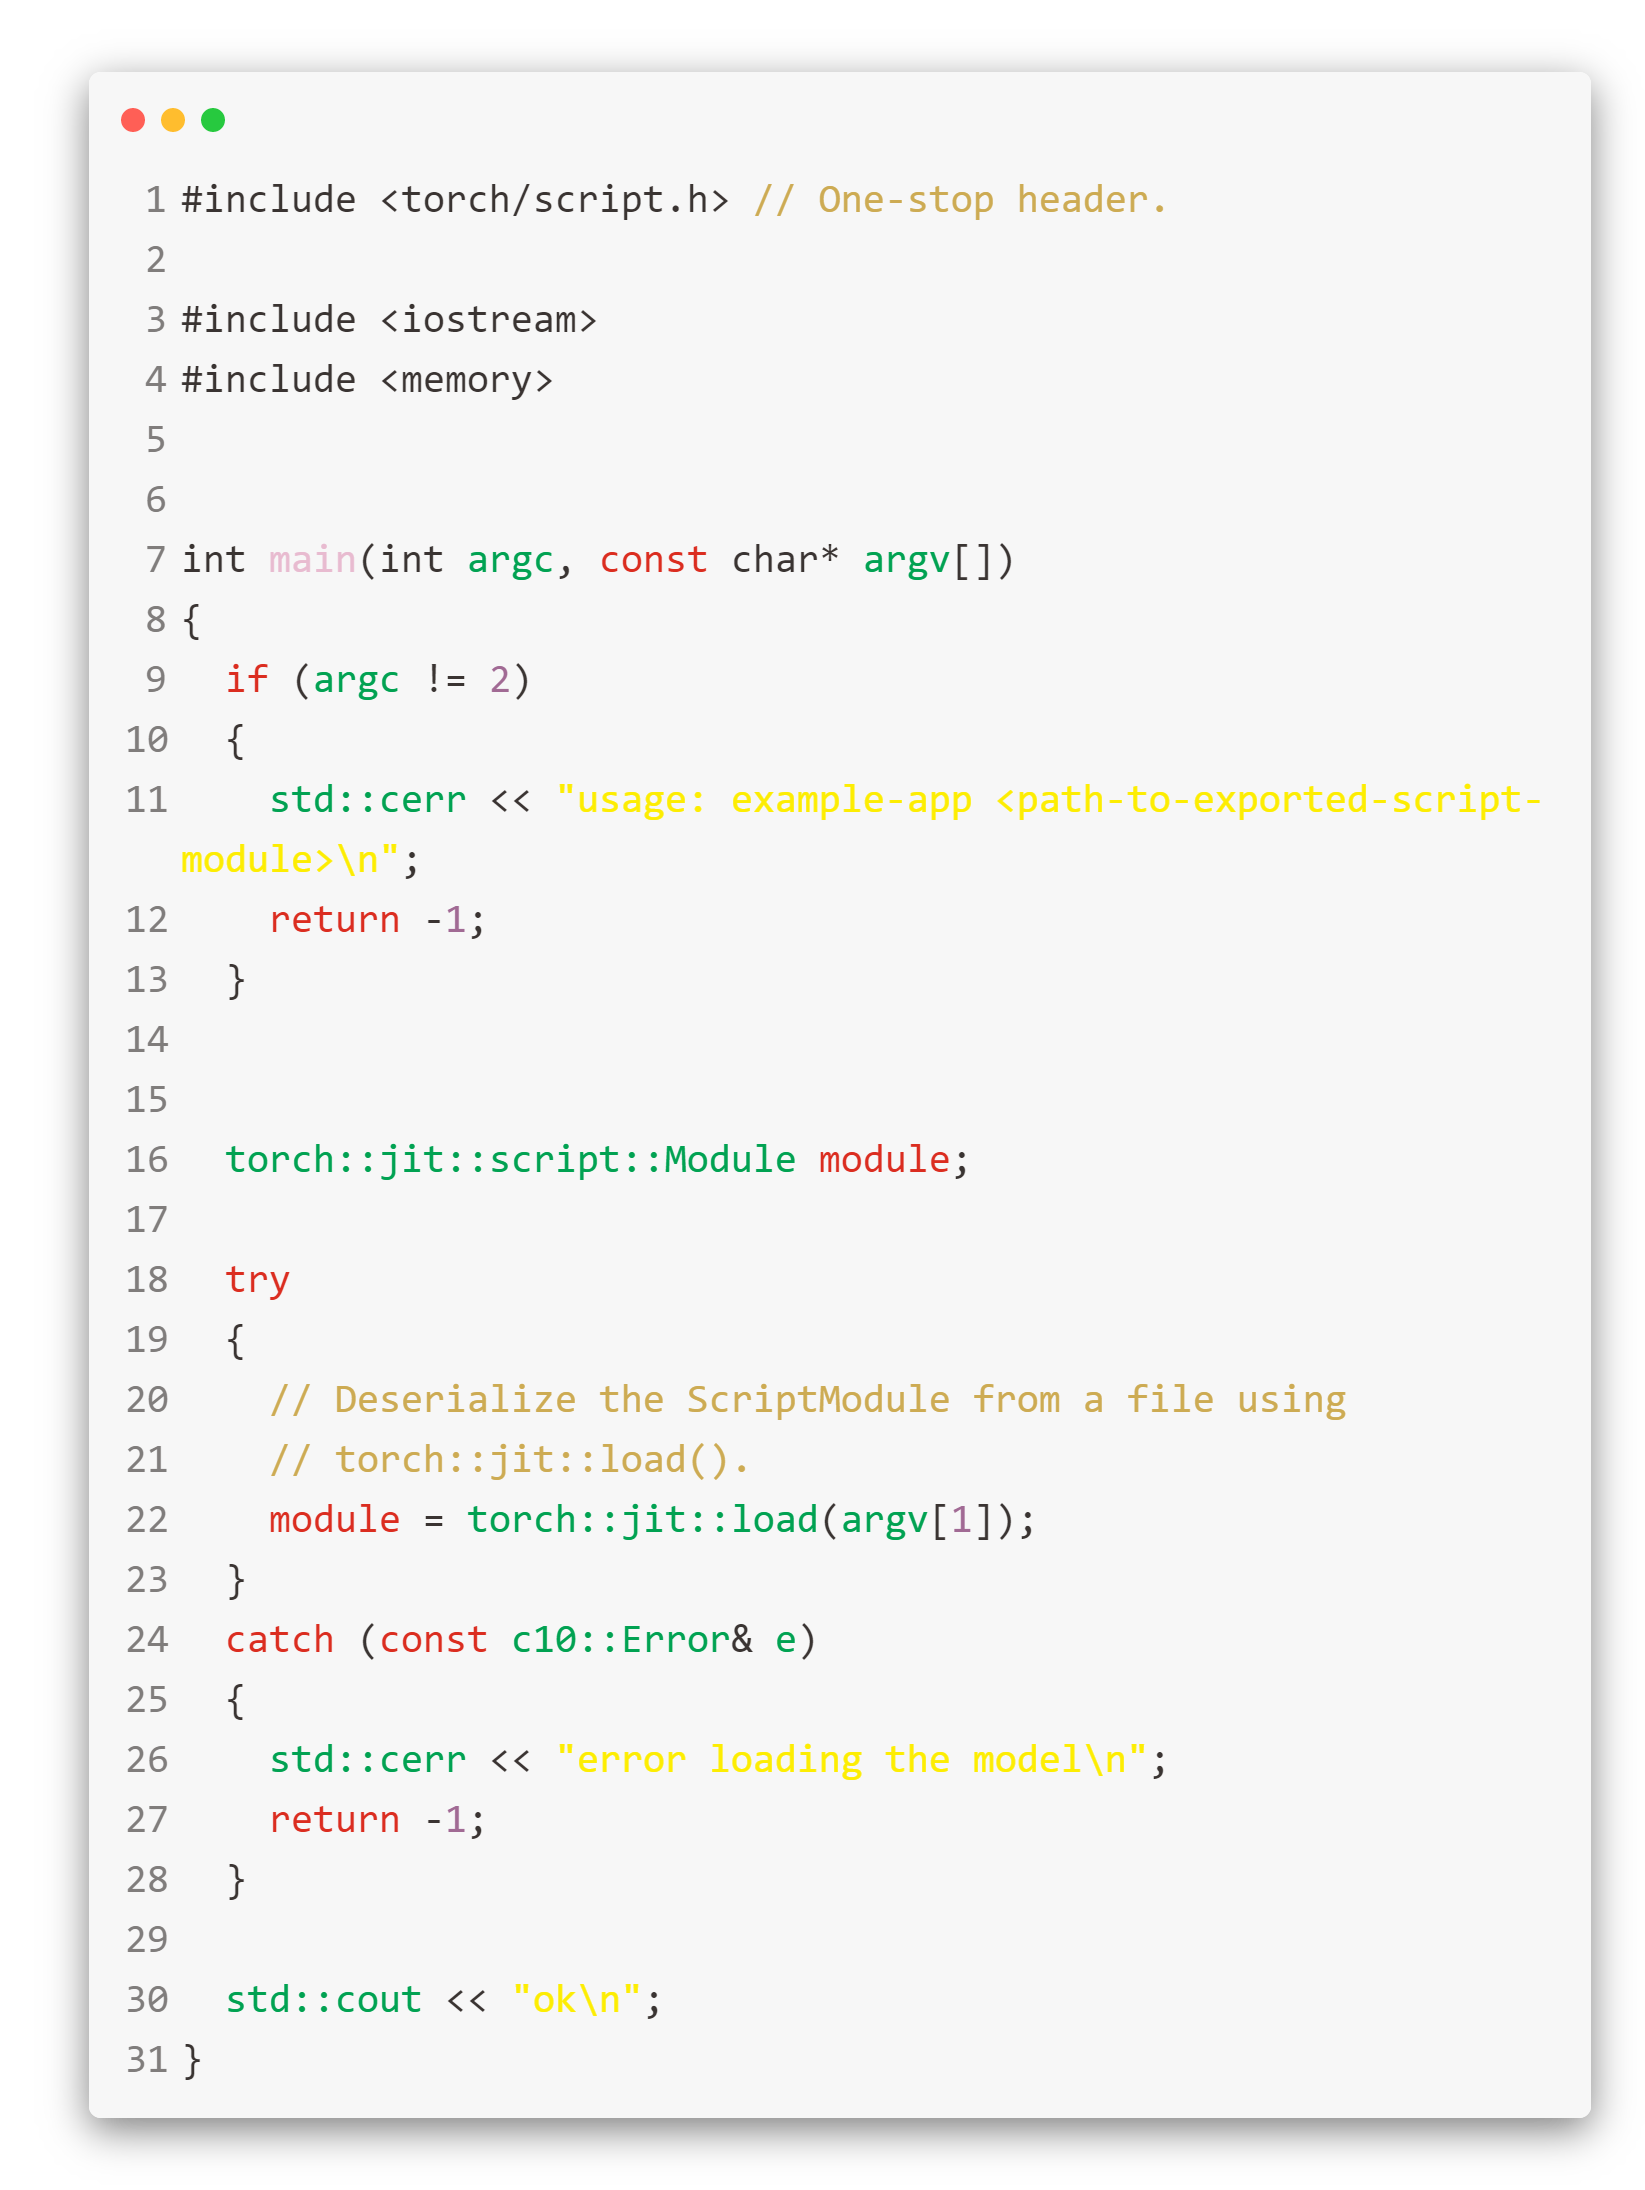
\includegraphics[width=0.98\linewidth]{figures/code-cpp-big.png}
%    \caption{Pytorch 模型在 C++ 项目中的应用}
%    \label{fig:code_cpp}
%\end{figure}

\pagebreak
\section{系统的部署与展示}\label{figures_tables}

介绍本文系统的部署与测试。本文的系统是运行于 Windows 平台,具体的运行环境见表~\ref{tab:env2}。在运行系统之前需要编译和配置好相关运行库,比如 LibTorch、OpenCV、MYNTAI S1040-IR-120/Mono的 SDK。

\subsection{系统运行环境}
本系统的开发和运行环境如表~\ref{tab:env1} 和表~\ref{tab:env2} 所示,包含软件环境和硬件环境。图~\ref{fig:photo} 展示的是本系统的真实硬件环境以及相应的系统交互界面。
\begin{table}[thbp]
	\centering
	\small\def\arraystretch{2.5}\setlength\tabcolsep{0.08\textwidth}
	\caption{系统开发环境}
	\begin{tabular}{|c|c|}
		\hline
		\multicolumn{2}{|c|}{软件环境}                \\
		\hline
		操作系统   & Ubuntu 18.04 \\
		\hline
		开发语言   & python、C++、matlab \\
		\hline
		运行环境  & python 3.6    \\
		\hline
		\multicolumn{2}{|c|}{硬件环境} \\
		\hline
		处理器    &      Intel(R) Core(TM) i5-4210U CPU @ 2.50 GHz  \\
		\hline
		内存      &       8GB         \\
		\hline
		显卡    &     TITAN X       \\
		\hline
	\end{tabular}
	\label{tab:env1}
\end{table}

\begin{table}[thbp]
	\centering
	\small\def\arraystretch{2.}\setlength\tabcolsep{0.05\textwidth}
	\caption{系统运行环境}
	\begin{tabular}{|c|c|}
		\hline
		\multicolumn{2}{|c|}{软件环境}                \\
		\hline
		操作系统   & Windows 10 					  \\
		\hline
		开发工具  & Matlab 2018b  					   \\
		\hline
		运行库   & LibTorch、OpenCV、MYNTAI S1040-IR-120/Mono SDK \\
		\hline
		\multicolumn{2}{|c|}{硬件环境} \\
		\hline
		处理器    &      Intel(R) Core(TM) i5-4210U CPU @ 2.50 GHz  \\
		\hline
		内存      &       8GB         \\
		\hline
		传感器    &     MYNTAI S1040-IR-120/Mono          \\
		\hline
	\end{tabular}
	\label{tab:env2}
\end{table}

\begin{figure}[htbp]
	\centering
	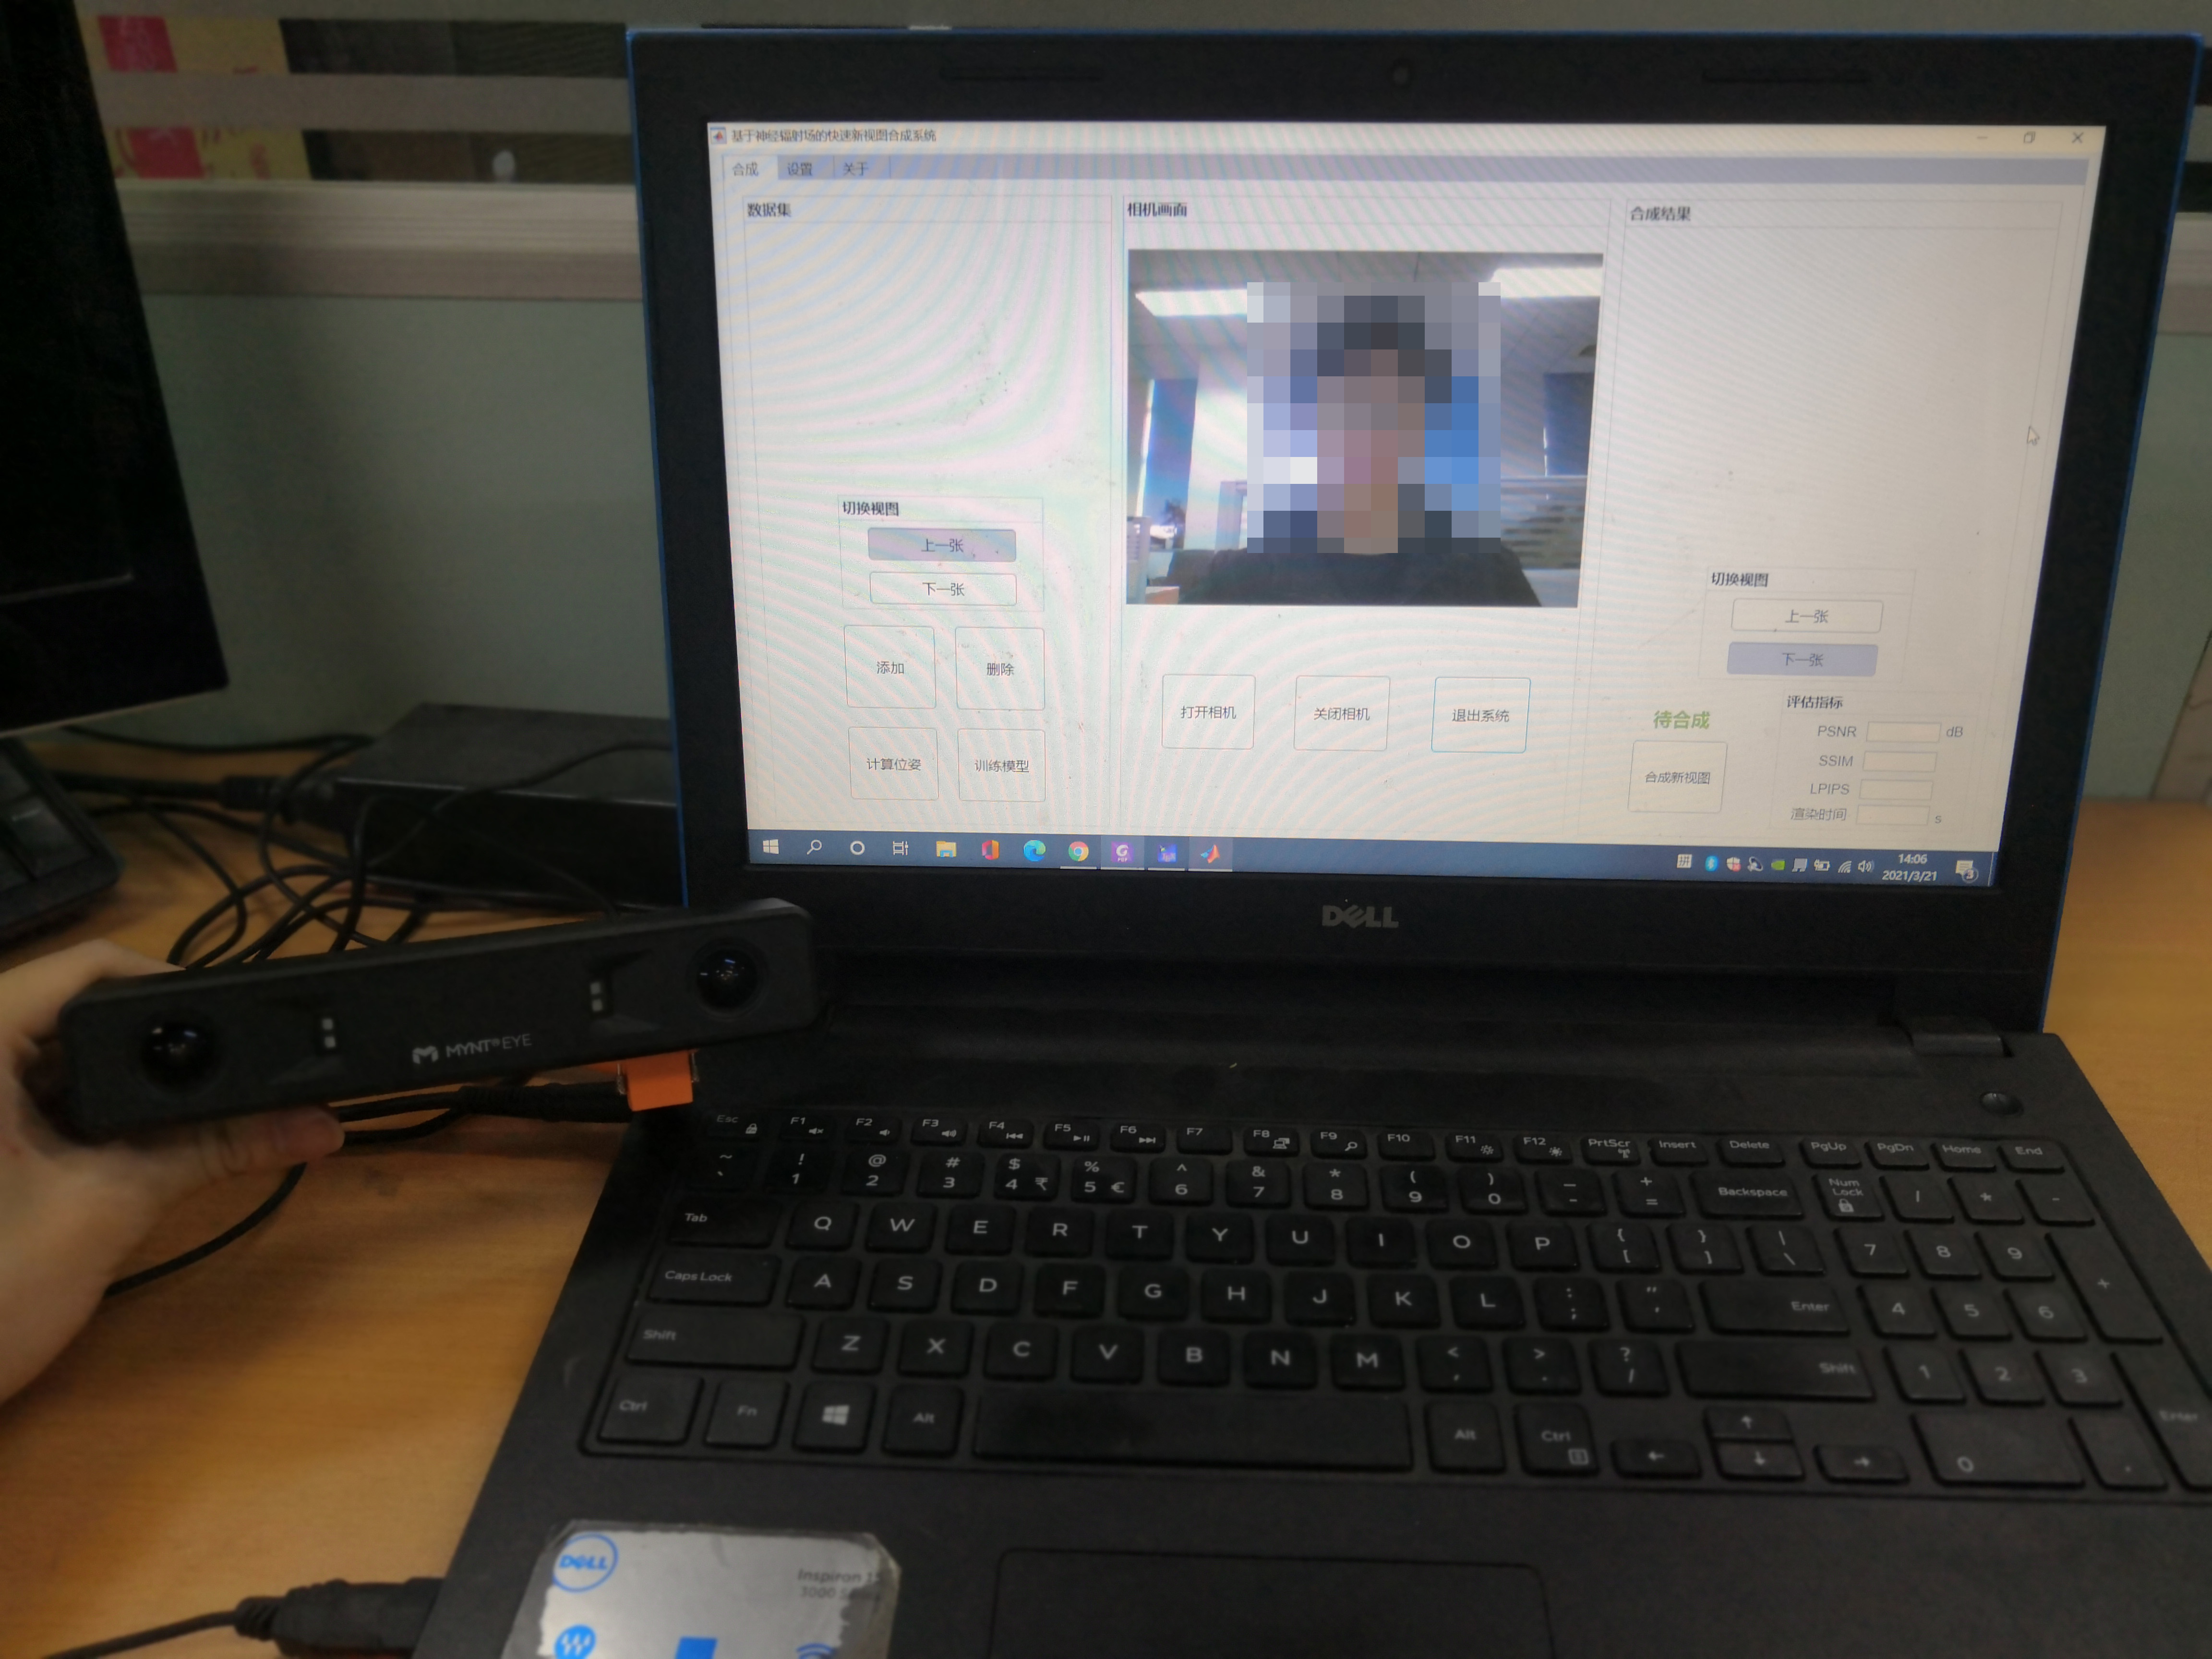
\includegraphics[width=0.85\linewidth]{figures/system-hardware.jpg}
	\caption{系统的硬件环境}
	\label{fig:photo}
\end{figure}
\pagebreak
\subsection{系统功能测试}
本小节针对本系统的各个模块进行测试,下面将详述测试的过程,并展示与用户交互的界面以及最终测试的结果。
\subsubsection{相机交互功能测试}
首先我们先测试电脑与相机方面的交互功能。与相机能够友好交互,获得稳定高质量的图像,这对整个训练或者测试都是意义重大地。相机传感器是数据的本源,是一切计算机视觉的基础和灵魂。拥有着一个鲁棒而友好的相机交互环境能为新视图合成任务提供非常好的输入,容易让网络学习到更准确的神经辐射场,预测出更准的颜色和体密度,这些都会在 PSNR、SSIM、LPIPS等指标上面体现出来。

\begin{table}[thbp]
	\centering
	\small\def\arraystretch{1.5}\setlength\tabcolsep{0.05\textwidth}
	\caption{相机交互功能测试用例}
	\begin{tabular}{|p{2cm}<{\centering}|p{4cm}<{\centering}|p{4cm}<{\centering}|}
		\hline
		用例编号 & \multicolumn{2}{|l|}{001}       \\
		\hline
		测试功能 & \multicolumn{2}{|l|}{相机交互}       \\
		\hline
		编号 & 输入/动作 & 期望结果 \\
		\hline
		1 & 打开应用,进入合成界面,在相机画面栏点击打开相机按钮 & 跳转到传感器 RGBD 相机界面 \\
		\hline
		2 & 在数据集栏点击添加按钮 & 当前相机的图像被捕获到数据集栏 \\
		\hline
		3 & 在相机画面栏点击关闭相机 & 提示:“您确定要关闭相机吗?” \\
		\hline
		4 & 点击确认关闭 & 相机画面终止 \\
		\hline
		5 & 点击取消关闭 & 整个交互界面不变 \\
		\hline
		6 & 点击退出系统 & 提示:“您确定退出吗?” \\
		\hline
		7 & 点击确认退出 & 整个交互界面退出 \\
		\hline
		8 & 点击取消退出 & 整个交互界面不变 \\
		\hline
	\end{tabular}
	\label{tab:camera}
\end{table}
根据表~\ref{tab:camera},整个数据集处理的测试步骤如下:
\begin{enumerate}
	\item[1)] 打开应用进入合成菜单栏,点击打开相机按钮,测试结果如图~\ref{fig:camara-a} 和图~\ref{fig:camara-b}。用例001编号为1的测试符合预期结果。
	\item[2)] 在数据集面板上点击添加,当前相机画面会被捕获到数据集,具体测试如图~\ref{fig:camara-c}。用例001编号为2的测试符合预期结果。
	\item[3)] 若点击了相机界面的关闭相机按钮,会有相应提示信息,如图~\ref{fig:camara-d} 所示。若点击是,则相机画面终止,如图~\ref{fig:camara-e} 所示。若点击否,则保持不变,如图~\ref{fig:camara-c}。用例001编号为3、4、5的测试符合预期结果。
	\item[4)] 若点击了相机界面的退出系统按钮,会有相应提示信息,如图~\ref{fig:camara-f} 所示。若点击是,则程序画面终止。若点击否,则保持不变,如图~\ref{fig:camara-e}。用例001编号为6、7、8的测试符合预期结果。
\end{enumerate}

\begin{figure}[bhtp]
	\centering
	\subcaptionbox{打开应用画面\label{fig:camara-a}}
	{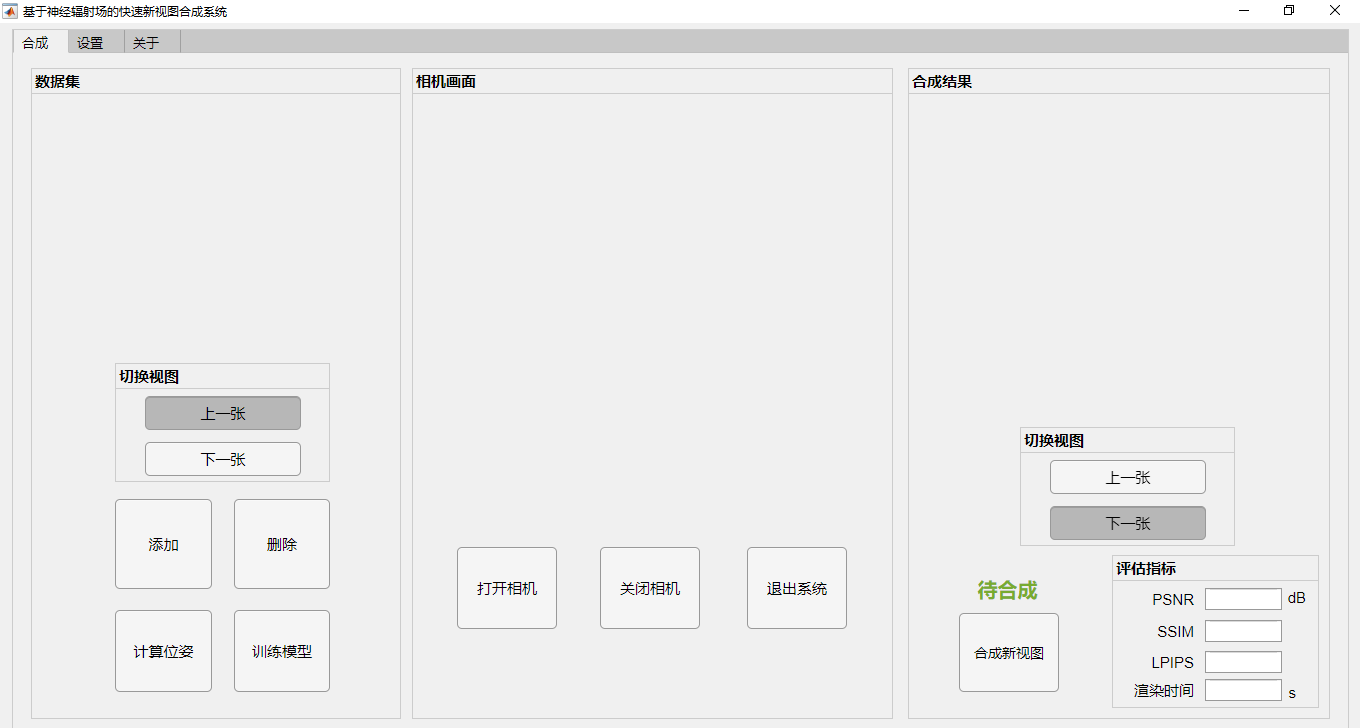
\includegraphics[width=0.45\linewidth]{figures/system/1-a.png}}
	\subcaptionbox{打开相机画面\label{fig:camara-b}}
	{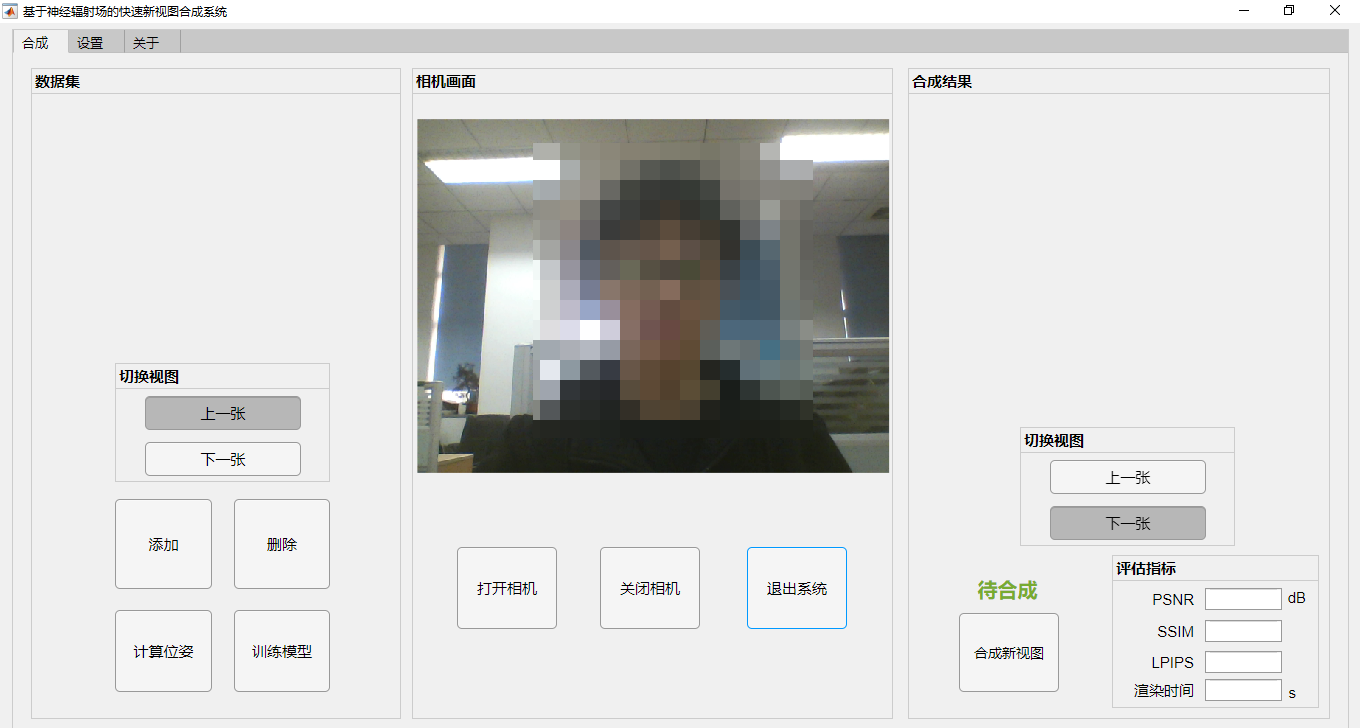
\includegraphics[width=0.45\linewidth]{figures/system/1-b.png}} \\
	\subcaptionbox{捕获相机画面\label{fig:camara-c}}
	{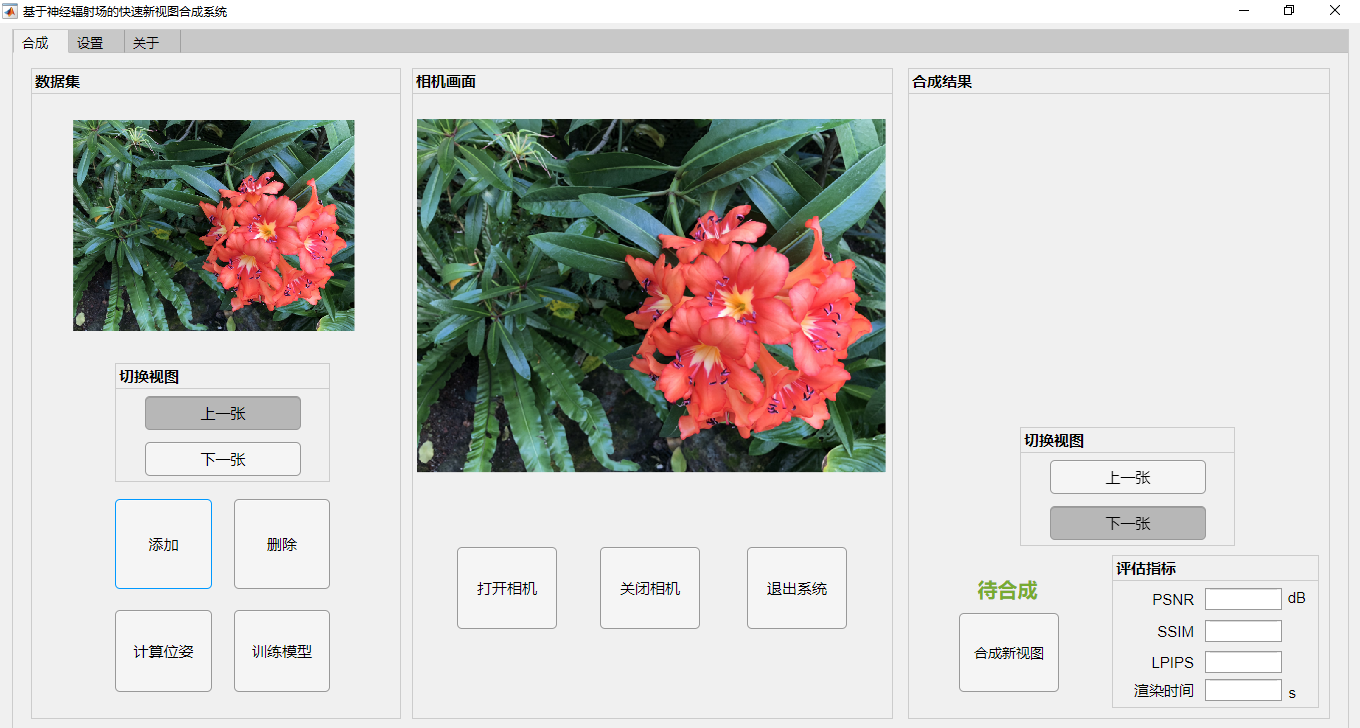
\includegraphics[width=0.45\linewidth]{figures/system/1-c.png}}
	\subcaptionbox{关闭相机提示信息\label{fig:camara-d}}
	{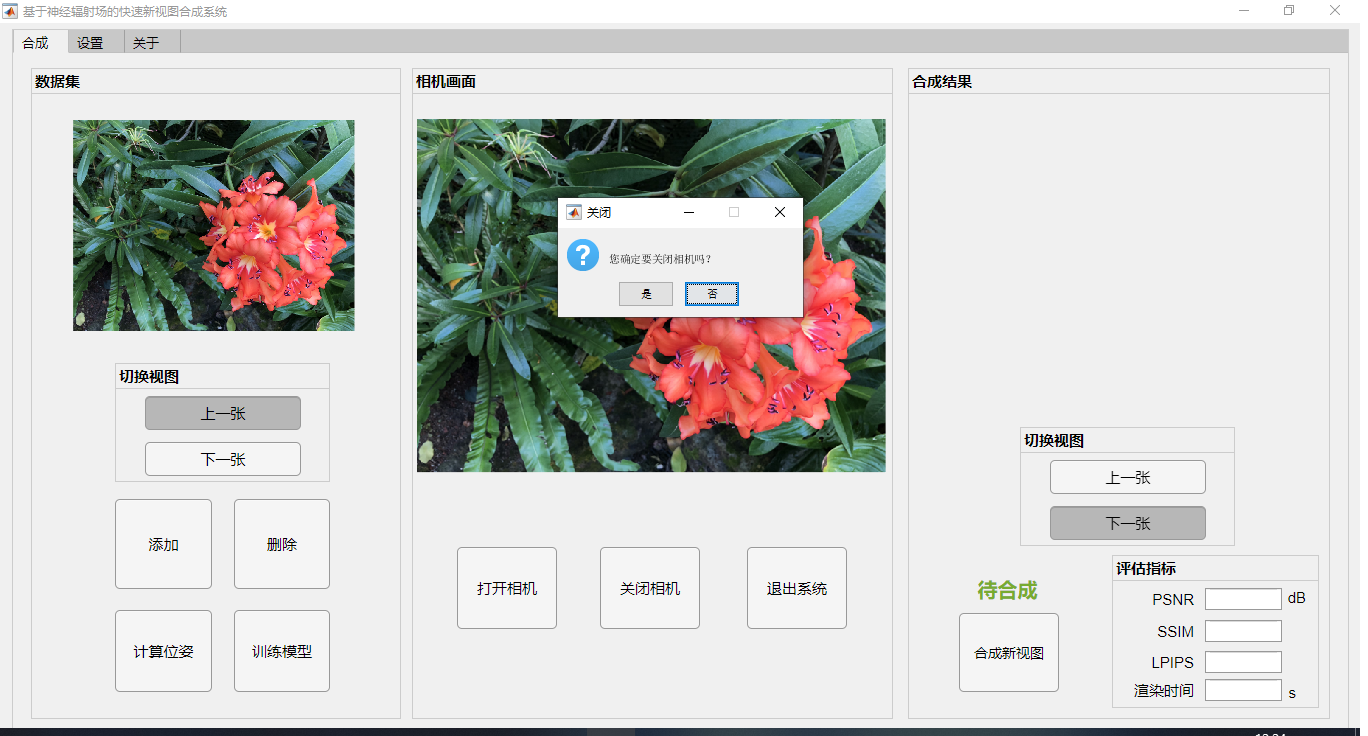
\includegraphics[width=0.45\linewidth]{figures/system/1-d.png}} \\
	\subcaptionbox{关闭相机画面\label{fig:camara-e}}
	{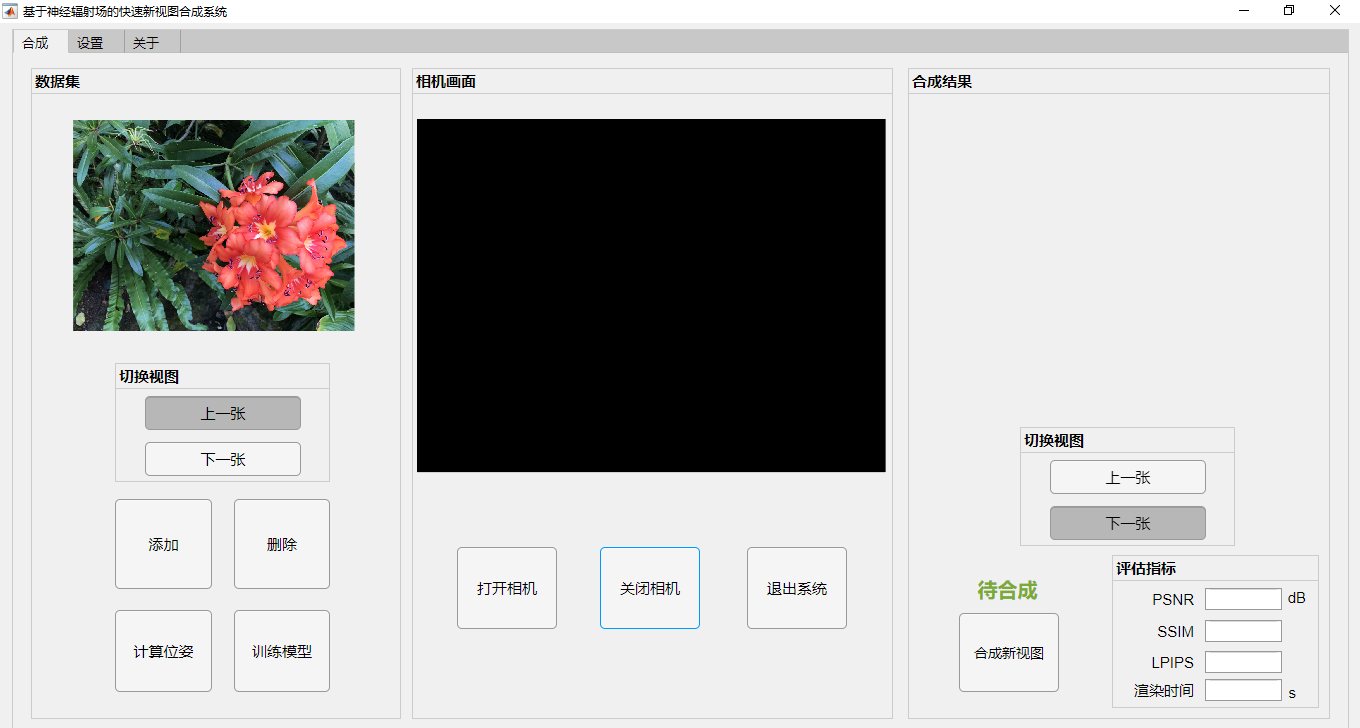
\includegraphics[width=0.45\linewidth]{figures/system/1-e.png}}
	\subcaptionbox{退出应用提示信息\label{fig:camara-f}}
	{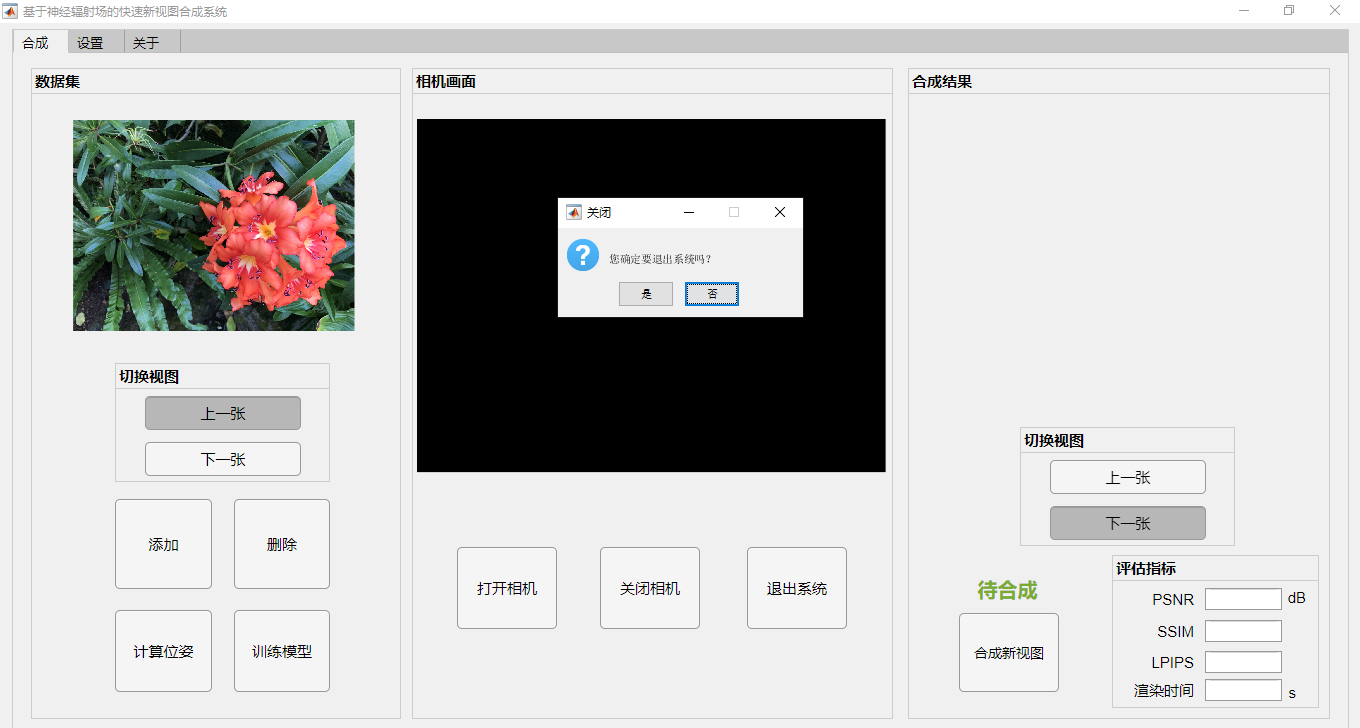
\includegraphics[width=0.45\linewidth]{figures/system/1-f.png}}
	\caption{相机交互功能测试}
	\label{fig:camara}
\end{figure}
\newpage

\subsubsection{数据集处理功能测试}
数据集处理是整个系统的最先使用的功能,非常至关重要,数据的选取决定了最终测试结果的好坏。数据集处理对应于本系统数据处理模块的功能。首先介绍下数据处理模块对应的典型测试用例,主要包含数据集的获取,删除。

\begin{table}[t]
	\centering
	\small\def\arraystretch{1.3}\setlength\tabcolsep{0.05\textwidth}
	\caption{数据集处理功能测试用例}
	\begin{tabular}{|p{2cm}<{\centering}|p{4cm}<{\centering}|p{4cm}<{\centering}|}
		\hline
		用例编号 & \multicolumn{2}{|l|}{002}       \\
		\hline
		测试功能 & \multicolumn{2}{|l|}{数据集处理}       \\
		\hline
		编号 & 输入/动作 & 期望结果 \\
		\hline
		1 & 打开应用,进入合成界面,在相机画面栏点击打开相机按钮 & 跳转到传感器 RGBD 相机界面 \\
		\hline
		2 & 在数据集栏点击添加按钮 & 当前相机的 RGB 数据被选作数据集并显示在数据集栏上 \\
		\hline
		3 & 在数据集栏点击上(下)一张按钮 & 数据集栏画面切换为上(下)一张图像 \\
		\hline
		4 & 在数据集栏点击删除按钮 & 提示:“您确定删除吗?” \\
		\hline
		5 & 点击确认删除 & 数据集栏当前显示的图像被删除 \\
		\hline
		6 & 点击取消删除或者提示栏右上角$\times$ & 数据集栏当前显示的图像被保留在数据集中 \\
		\hline
	\end{tabular}
	\label{tab:getdataset}
\end{table}

根据表~\ref{tab:getdataset},整个数据集处理的测试步骤如下:
\begin{enumerate}
	\item[1)] 打开应用进入合成菜单栏,点击打开相机按钮,测试结果如图~\ref{fig:camara-b}。用例002编号为1的测试与预期结果相符。
	\item[2)] 在数据集面板上点击添加,当前相机画面会被捕获到数据集,如图~\ref{fig:camara-c}。用例002编号为2的测试符合预期结果。
	\item[3)] 若点击数据集栏上(下)一张按钮,视图会切换到上(下)一张图像,如图~\ref{fig:datasetProcess-a} 和图~\ref{fig:datasetProcess-b}。用例002编号为3的测试符合预期结果。
	\item[4)] 若在数据集栏点击了删除按钮,会有相应提示信息,如图~\ref{fig:datasetProcess-c}。若点击是,则数据集当前画面终止,如图~\ref{fig:datasetProcess-d} 所示。若点击否,则保持不变,如图~\ref{fig:camara-e}。用例002编号为4、5、6的测试符合预期结果。
\end{enumerate}
\pagebreak
\begin{figure}[thbp]
	\centering 
	% 0.55
	\subcaptionbox{上一张捕获图像\label{fig:datasetProcess-a}}
	{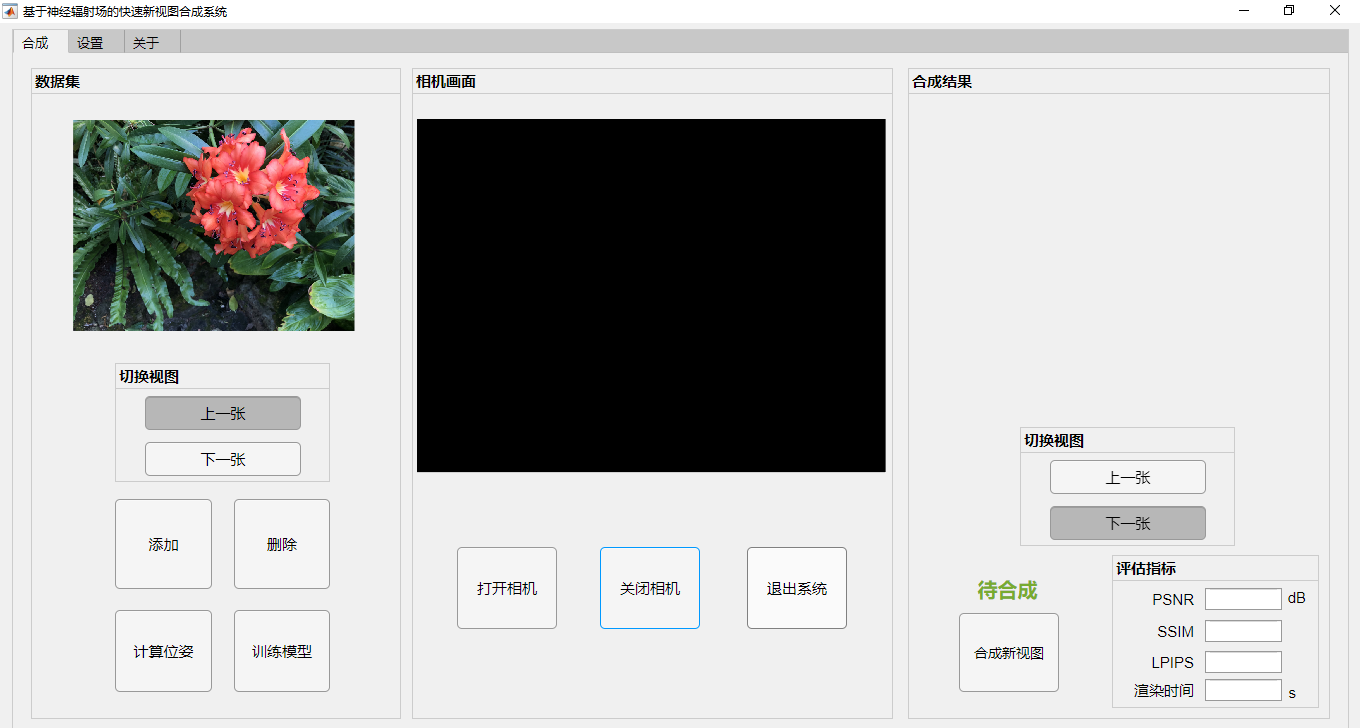
\includegraphics[width=0.45\linewidth]{figures/system/2-a.png}}
	\subcaptionbox{下一张捕获图像\label{fig:datasetProcess-b}}
	{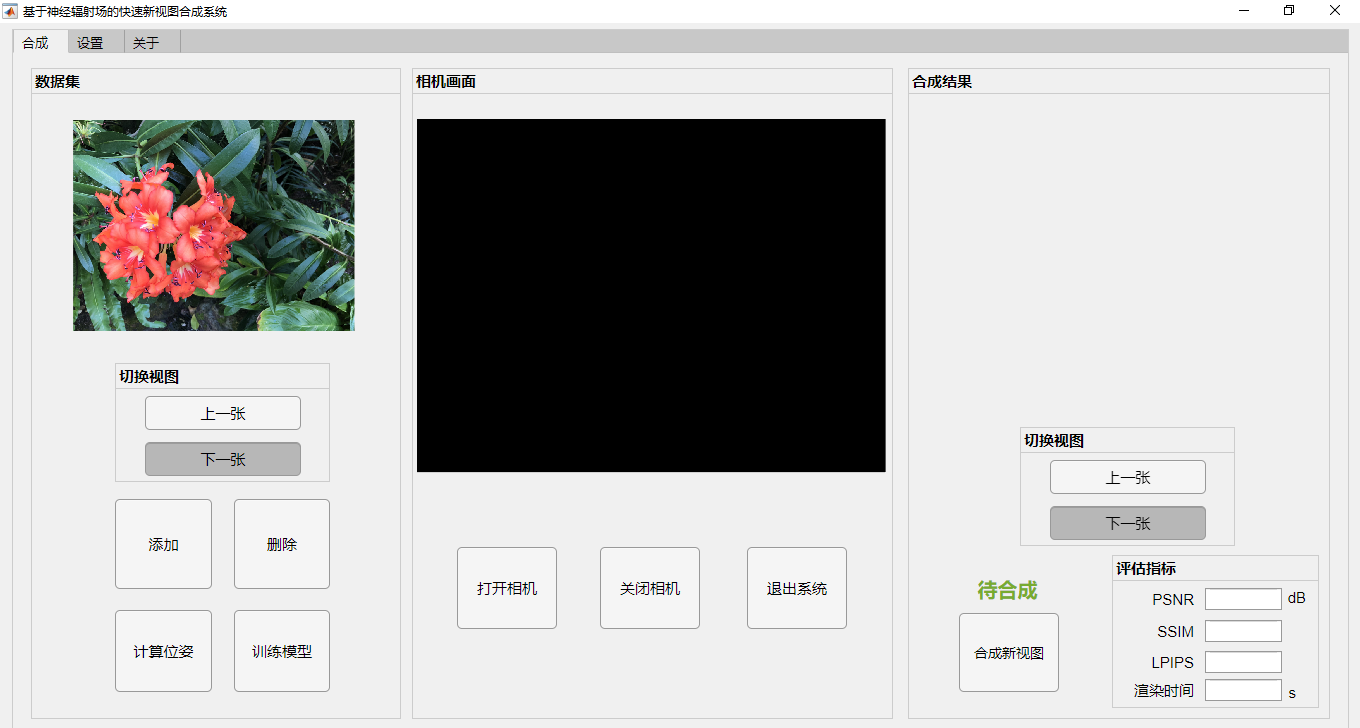
\includegraphics[width=0.45\linewidth]{figures/system/2-b.png}}
	\subcaptionbox{删除数据的提示信息\label{fig:datasetProcess-c}}
	{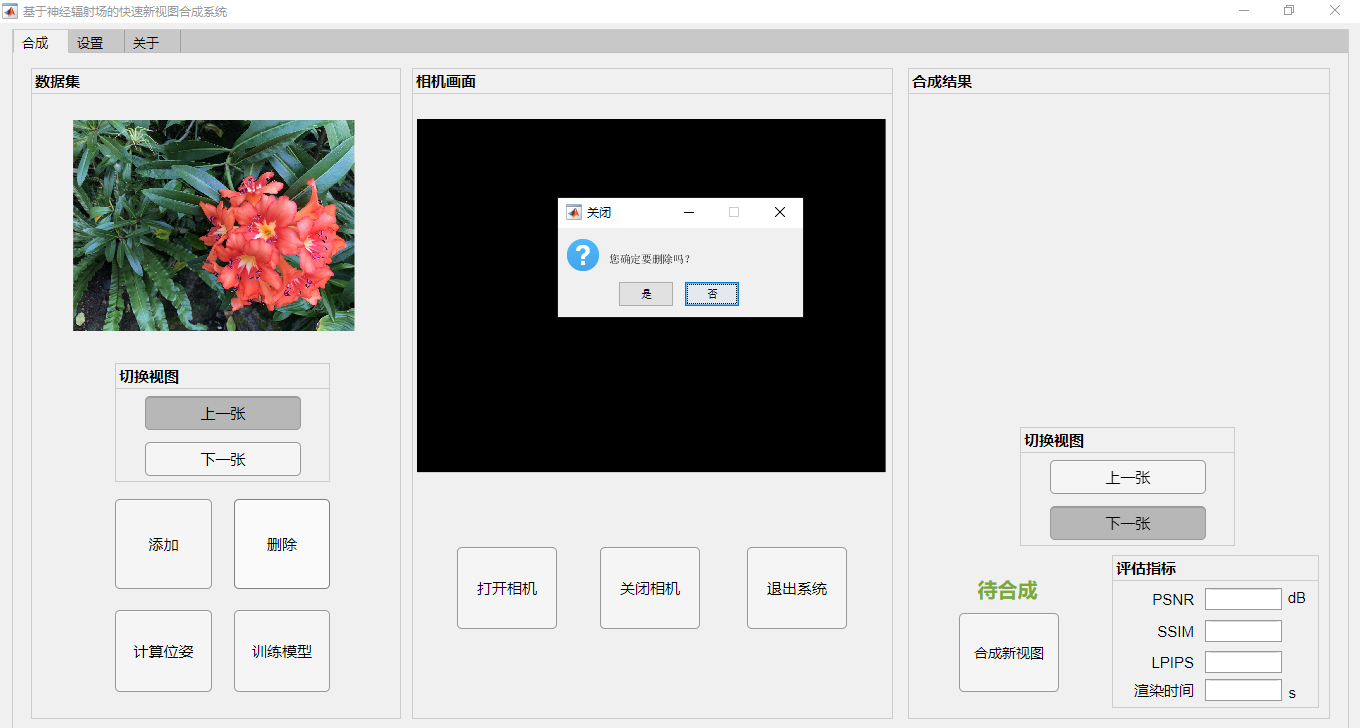
\includegraphics[width=0.45\linewidth]{figures/system/2-c.png}}
	\subcaptionbox{删除后的画面\label{fig:datasetProcess-d}}
	{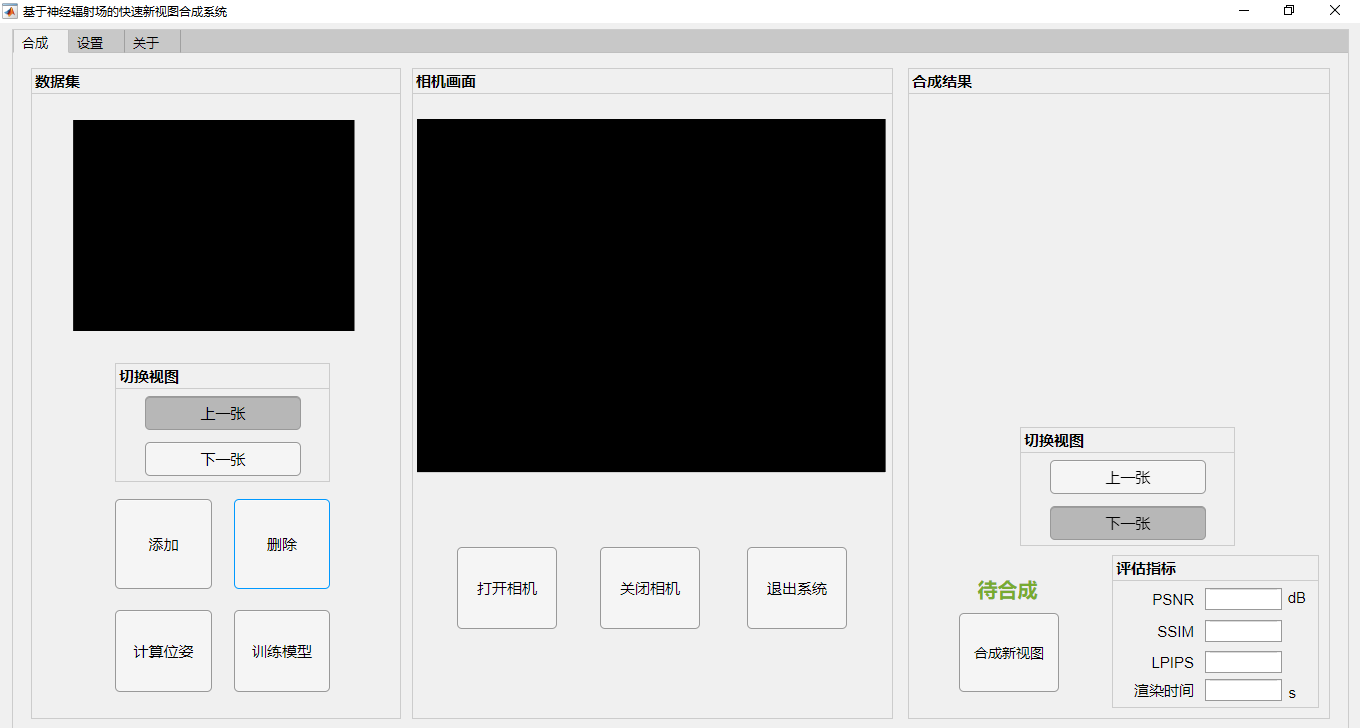
\includegraphics[width=0.45\linewidth]{figures/system/2-d.png}}
	\caption{数据集处理功能测试}
	\label{fig:datasetProcess}
\end{figure}

\begin{table}[htbp]
	\centering
	\small\def\arraystretch{0.9}\setlength\tabcolsep{0.05\textwidth}
	\caption{新视图合成功能测试用例}
	\begin{tabular}{|p{2cm}<{\centering}|p{4cm}<{\centering}|p{4cm}<{\centering}|}
		\hline
		用例编号 & \multicolumn{2}{|l|}{003}       \\
		\hline
		测试功能 & \multicolumn{2}{|l|}{新视图合成}       \\
		\hline
		编号 & 输入/动作 & 期望结果 \\
		\hline
		1 & 点击计算位姿按钮 &  进度条提示计算位姿的过程 \\
		\hline
		2 & 点击训练模型按钮 &  进度条提示模型训练的过程 \\
		\hline
		3 & 点击合成新视图按钮 & 状态提示从待合成到合成中再到已合成 \\
		\hline
		4 & 在合成栏点击上(下)一张按钮 & 数据集栏画面切换为上(下)一张图像,并显示相应的指标信息 \\
		\hline
	\end{tabular}
	\label{tab:viewsynthesis}
\end{table}
\subsubsection{新视图合成功能测试}
基于之前的功能测试,对于本系统的任务来说并不够,因为还没有检验本文方法的可行性与效率。基于神经辐射场的快速新视图合成,最终必须落脚于新视图合成,并对其进行加速。为了和之前保持一致,本系统在训练和测试环节都使用 $504 \times 378$ 的图像。下面是整个系统的最后一部分测试,是为了检测本文整个方法的性能,包含渲染速度以及渲染质量(包含PSNR、SSIM、LPIPS)等指标。通过多方面去表征本系统能有效地对 NeRF 进行加速,加速后的合成视图界面大图如图~\ref{fig:viewsynthesisBig} 所示。
%\begin{table}[htbp]
%	\centering
%	\small\def\arraystretch{1.}\setlength\tabcolsep{0.05\textwidth}
%	\caption{新视图合成功能测试用例}
%	\begin{tabular}{|p{2cm}<{\centering}|p{4cm}<{\centering}|p{4cm}<{\centering}|}
%		\hline
%		用例编号 & \multicolumn{2}{|l|}{003}       \\
%		\hline
%		测试功能 & \multicolumn{2}{|l|}{新视图合成}       \\
%		\hline
%		编号 & 输入/动作 & 期望结果 \\
%		\hline
%		1 & 点击计算位姿按钮 &  进度条提示计算位姿的过程 \\
%		\hline
%		2 & 点击训练模型按钮 &  进度条提示模型训练的过程 \\
%		\hline
%		3 & 点击合成新视图按钮 & 状态提示从待合成到合成中再到已合成 \\
%		\hline
%		4 & 在合成栏点击上(下)一张按钮 & 数据集栏画面切换为上(下)一张图像,并显示相应的指标信息 \\
%		\hline
%	\end{tabular}
%	\label{tab:viewsynthesis}
%\end{table}
根据表~\ref{tab:viewsynthesis},整个新视图功能测试的详细步骤如下:
\begin{enumerate}
	\item[1)] 若点击计算位姿按钮,会有相应提示信息,如图~\ref{fig:viewsynthesis-a} 和图~\ref{fig:viewsynthesis-b} 所示。用例003编号为1的测试与预期结果相符。
	\item[2)] 若点击训练模型按钮,会有相应提示信息,如图~\ref{fig:viewsynthesis-c} 和图~\ref{fig:viewsynthesis-d} 所示。用例003编号为2的测试与预期结果相符。
	\item[3)] 若点击合成新视图按钮,会有标签提示进度,如图~\ref{fig:viewsynthesis-e} 和图~\ref{fig:viewsynthesis-f} 以及图\ref{fig:viewsynthesis-g}。用例003编号为3的测试与预期结果相符。
	\item[4)] 若点击数据集栏上(下)一张按钮,视图会切换到上(下)一张图像,并且会显示本文 F-NeRF 合成新视角下图像的渲染质量信息和渲染时间信息,其中质量包含 PSNR、SSIM、LPIPS。如图~\ref{fig:viewsynthesis-h}(上)和图~\ref{fig:viewsynthesis-g}(下)所示,渲染时间分别为\SI{4.23}{s}和\SI{4.33}{s}。用例002编号为4的测试与预期结果相符。
\end{enumerate}



\begin{figure}[bhtp]
	\centering
	\subcaptionbox{提示信息,计算位姿中\label{fig:viewsynthesis-a}}
	{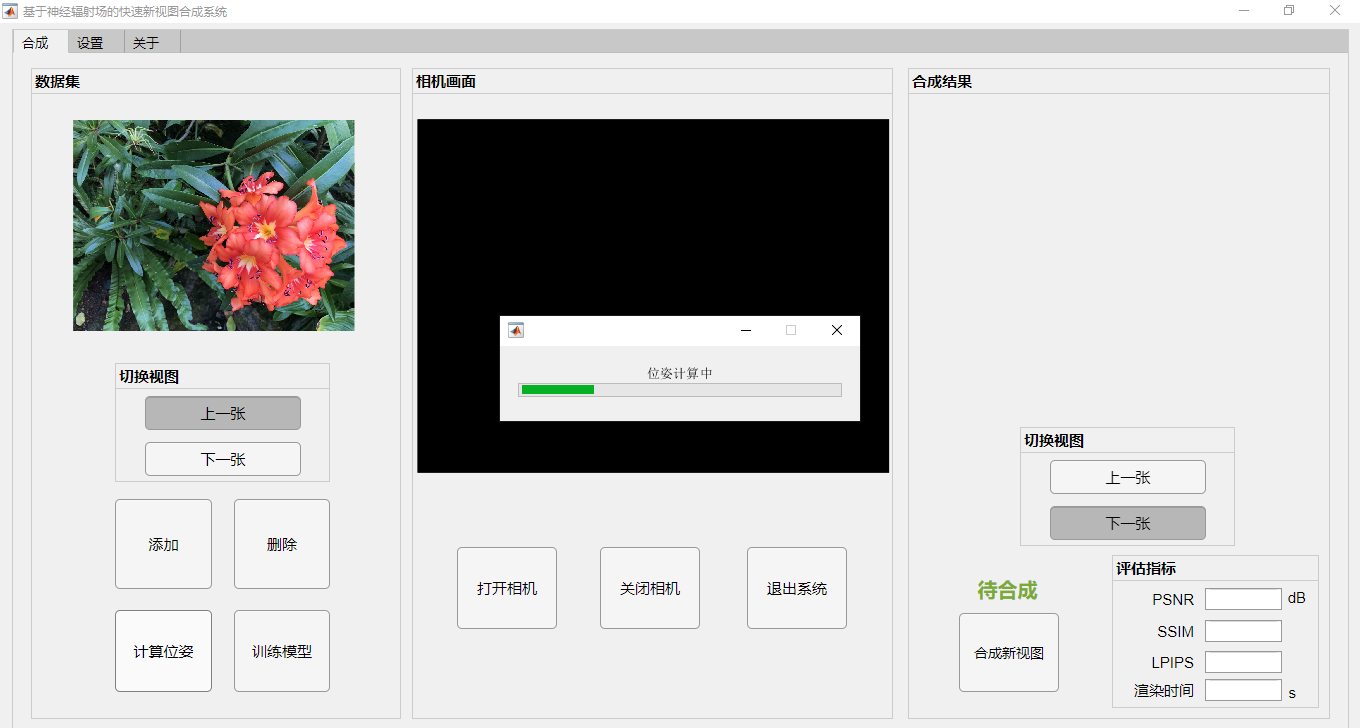
\includegraphics[width=0.45\linewidth]{figures/system/3-a.png}}
	\subcaptionbox{提示信息,计算位姿结束\label{fig:viewsynthesis-b}}
	{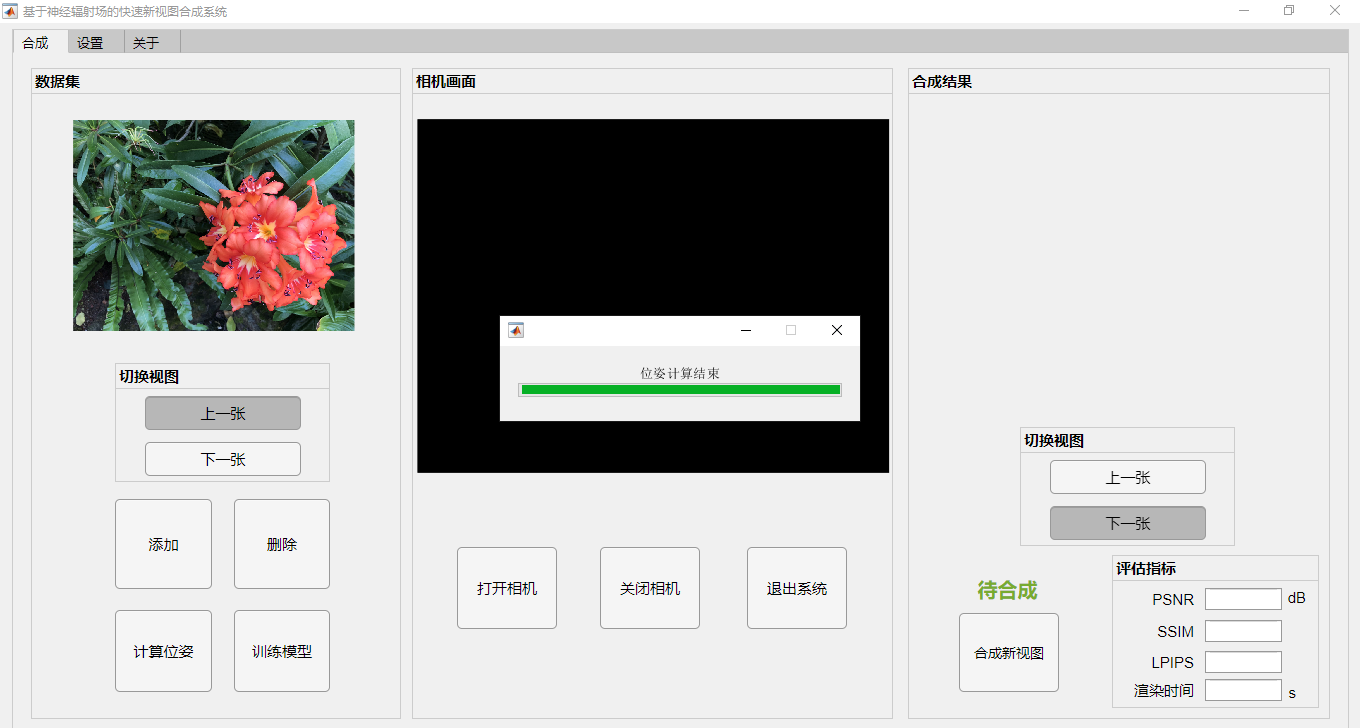
\includegraphics[width=0.45\linewidth]{figures/system/3-b.png}}
	\subcaptionbox{提示信息,训练中\label{fig:viewsynthesis-c}}
	{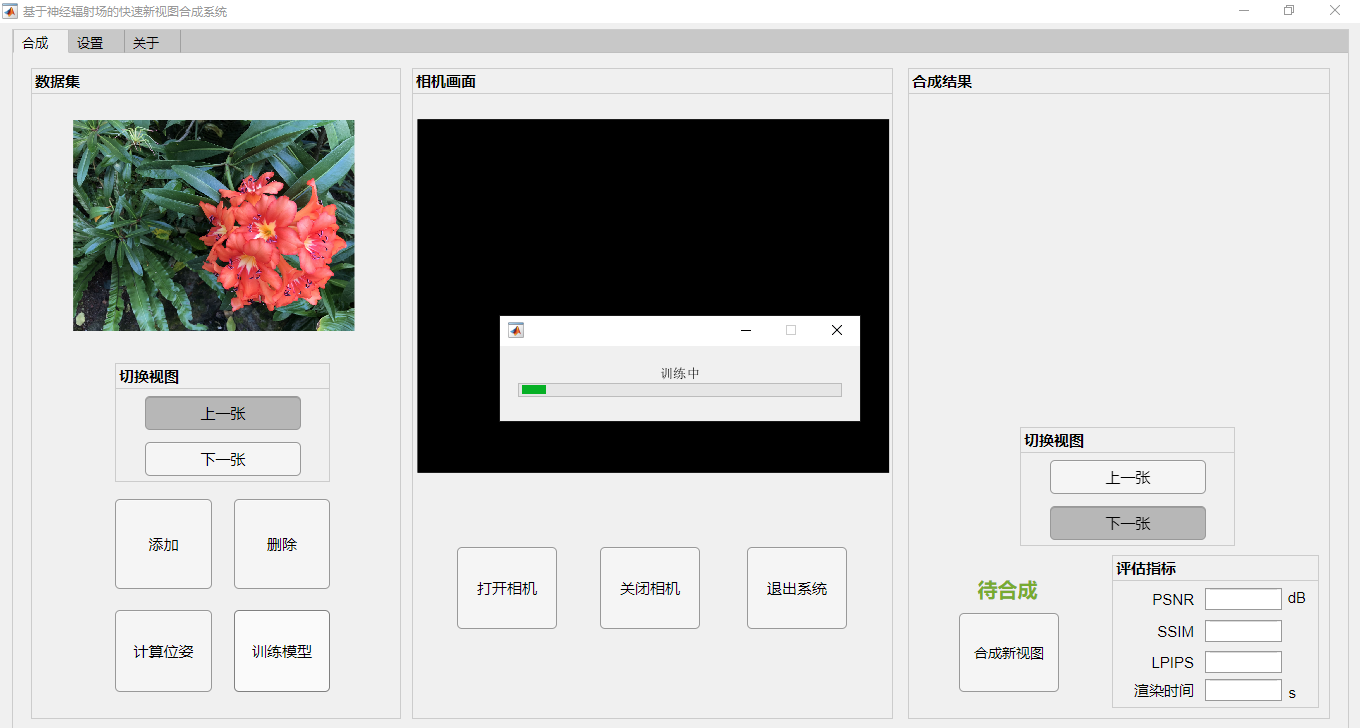
\includegraphics[width=0.45\linewidth]{figures/system/3-c.png}}
	\subcaptionbox{提示信息,训练结束\label{fig:viewsynthesis-d}}
	{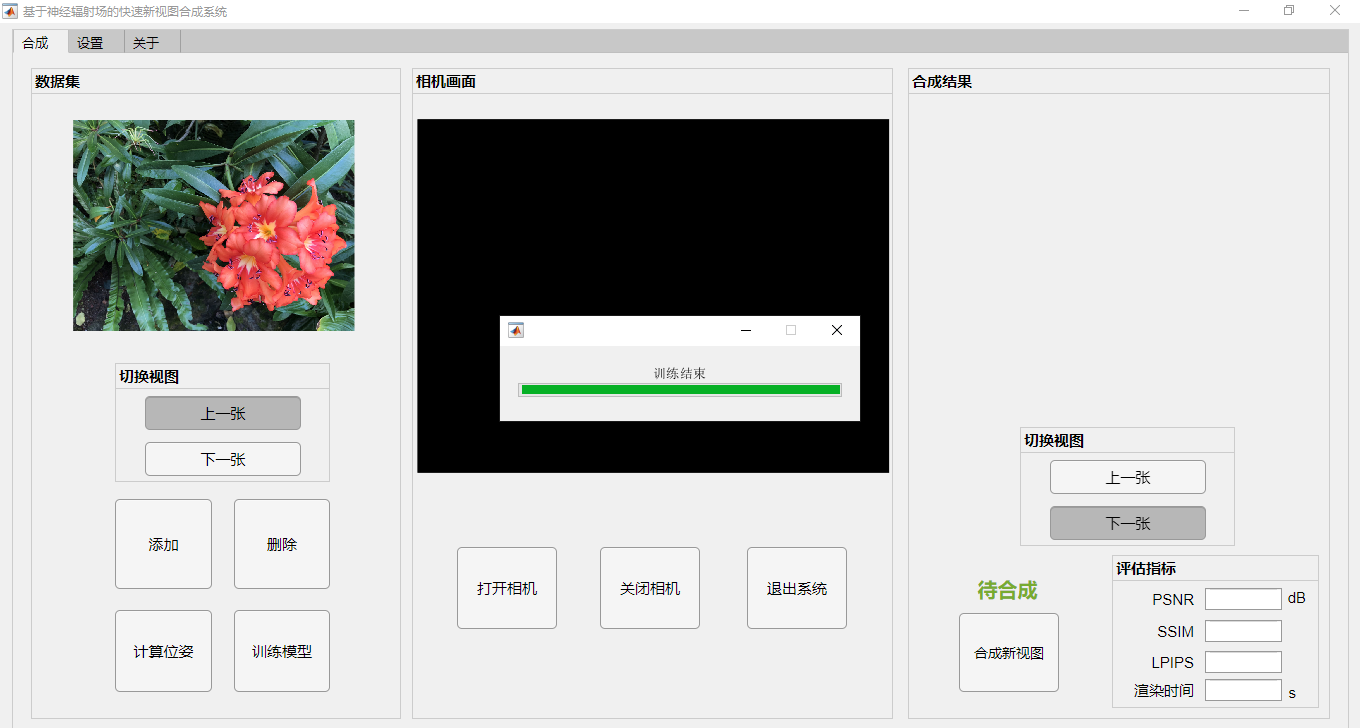
\includegraphics[width=0.45\linewidth]{figures/system/3-d.png}}
	\subcaptionbox{状态信息,待合成\label{fig:viewsynthesis-e}}
	{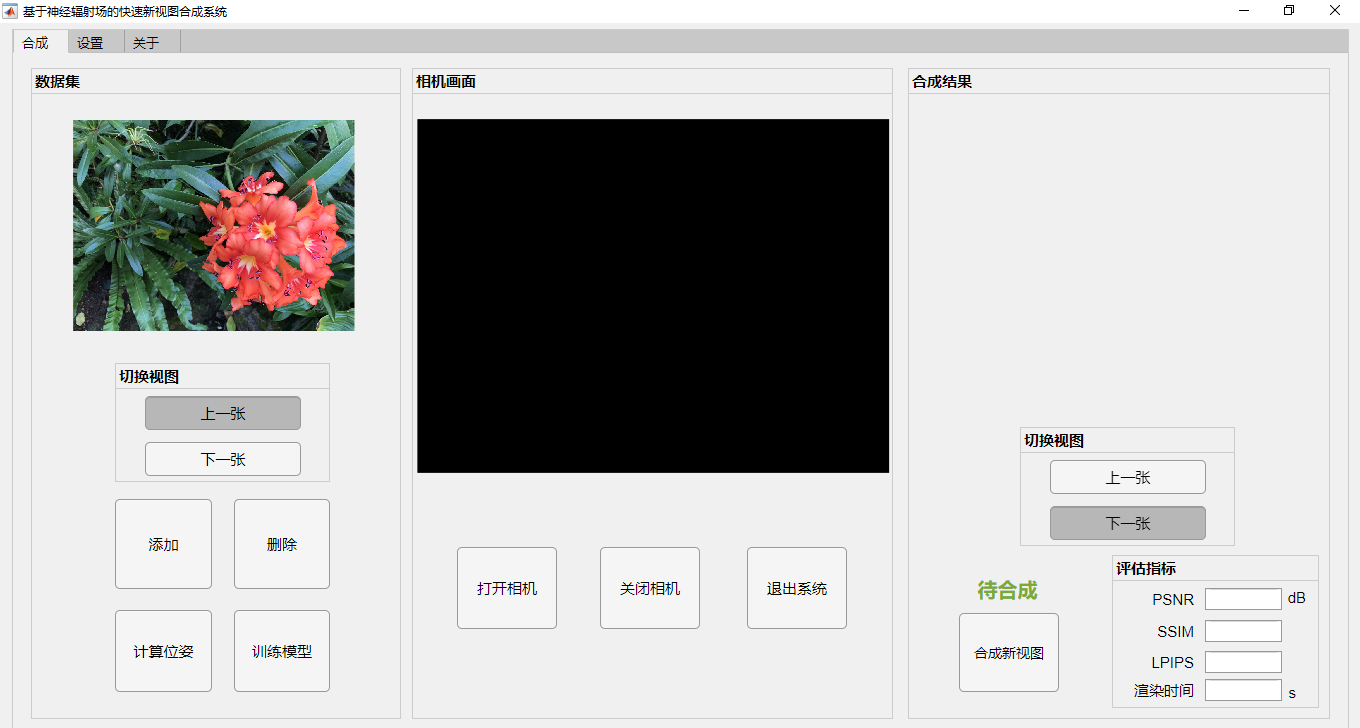
\includegraphics[width=0.45\linewidth]{figures/system/3-e.png}}
	\subcaptionbox{状态信息,合成中\label{fig:viewsynthesis-f}}
	{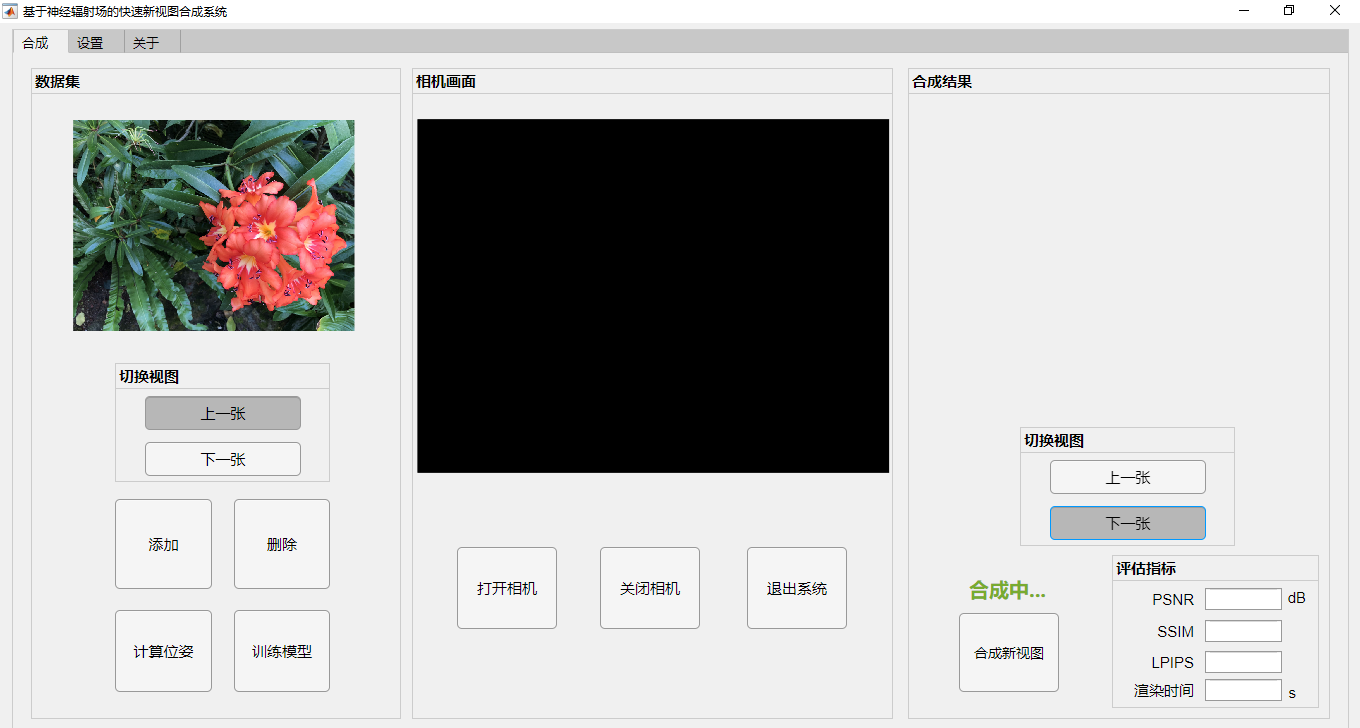
\includegraphics[width=0.45\linewidth]{figures/system/3-f.png}}
	\caption{新视图合成功能测试}
\end{figure}
\pagebreak
\begin{figure}[bhtp]
	\ContinuedFloat
	\centering
	\subcaptionbox{切换上一张已合成视图\label{fig:viewsynthesis-g}}
	{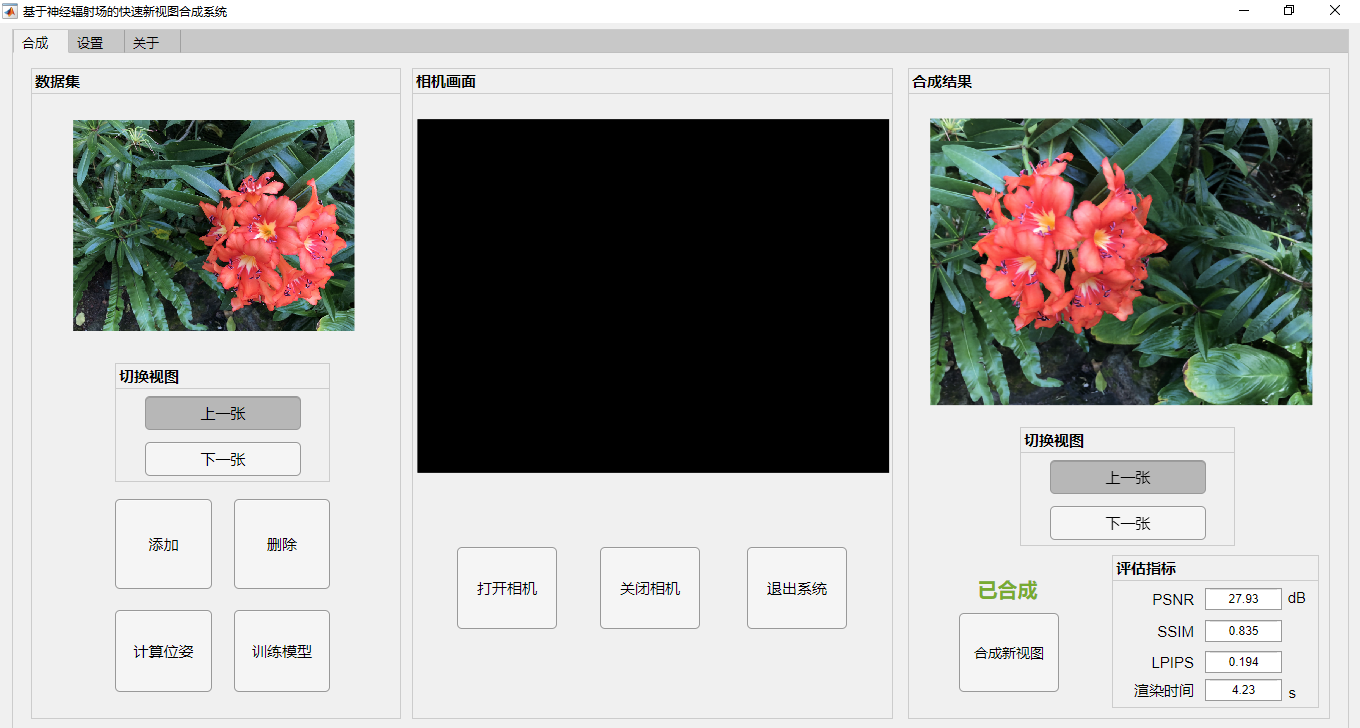
\includegraphics[width=0.45\linewidth]{figures/system/3-g.png}}
	\subcaptionbox{切换下一张已合成视图\label{fig:viewsynthesis-h}}
	{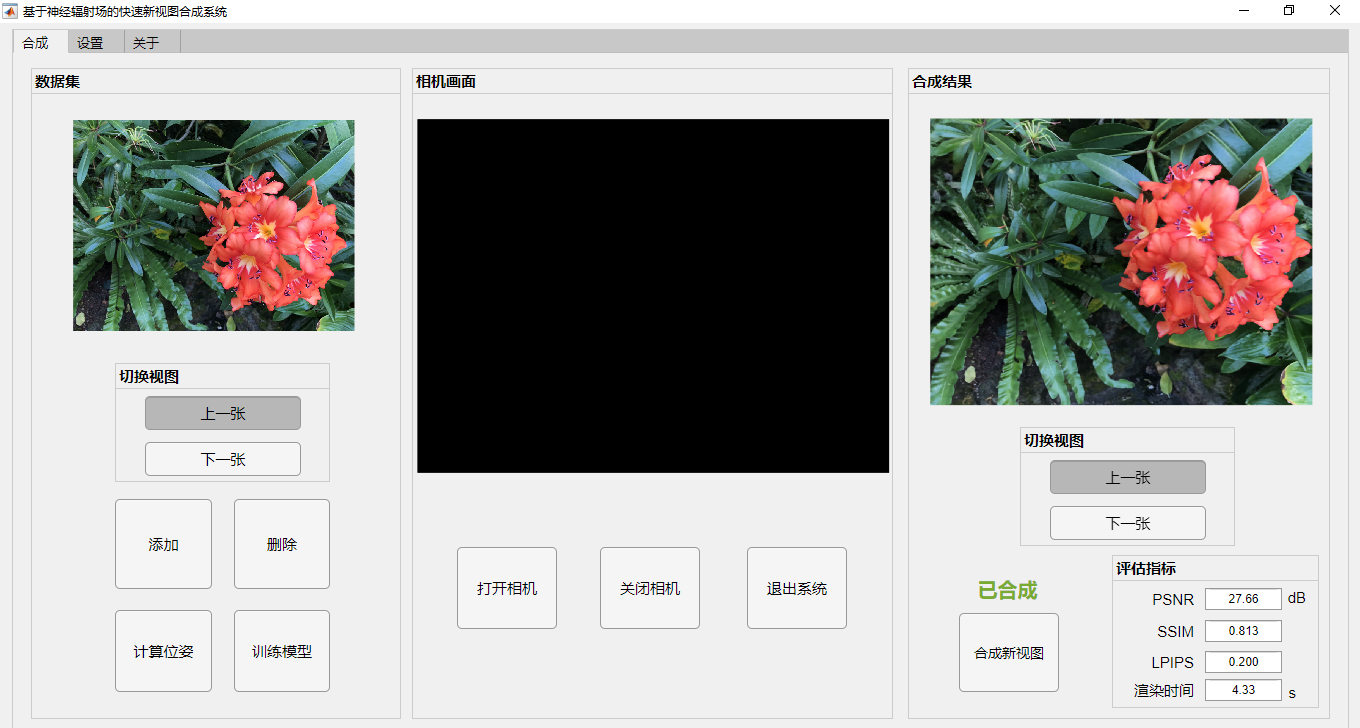
\includegraphics[width=0.45\linewidth]{figures/system/3-h.png}}
	\caption{(续) 新视图合成功能测试}
	\label{fig:viewsynthesis}
\end{figure}

\begin{figure}[htbp]
	\centering
	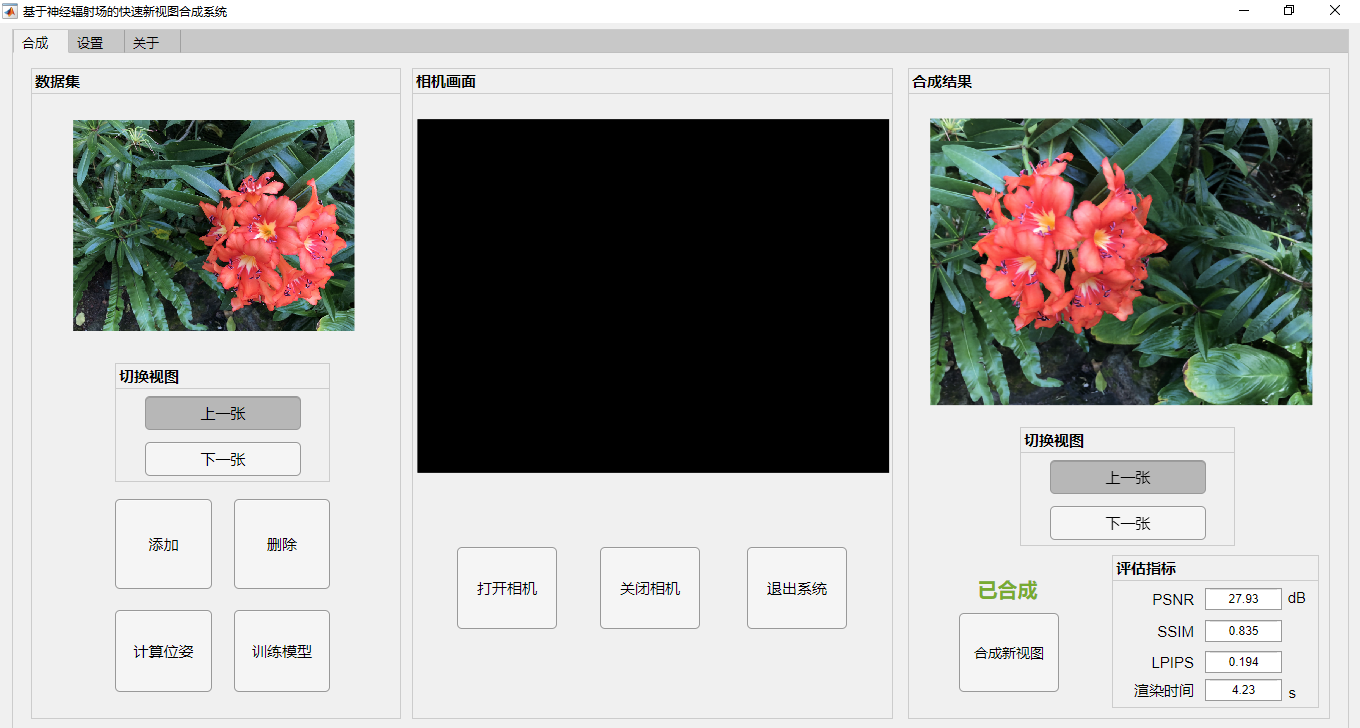
\includegraphics[width=0.95\linewidth]{figures/system/3-g.png}
	\caption{已合成的新视图,其中渲染时间为 \SI{4.23}{s}。}
	\label{fig:viewsynthesisBig}
\end{figure}
\section{本章小结}
本章主要介绍了基于神经辐射场的新视图快速合成系统的设计与实现。首先介绍了系统需求分析,包含功能性需求分析和非功能性需求分析,并展示了主要用例分析。然后阐述了此系统的基本设计架构以及将基于神经辐射场的新视图快速合成模型移植到 C++ 代码上的方法。之后介绍了系统的开发与运行环境。详尽地说明了经典测试用例的步骤,根据用例步骤完成了功能测试。从测试结果看,系统各项功能均能正常运行,合成新视图速度快且质量高。下一章将会对全文进行总结。
%本章主要介绍了基于神经辐射场的新视图快速合成系统的设计与实现。首先介绍了系统需求分析,并展示了主要用例分析。然后阐述了此系统的基本设计架构以及将本文的模型移植到 C++ 代码上的方法。之后介绍了系统的开发与运行环境。详尽地说明了经典测试用例的步骤,根据用例步骤完成了功能测试。从测试结果看,系统各项功能均能正常运行,合成新视图速度快且质量高。

\cleardoublepage
